%!TEX root = ../TAMUTemplate.tex
%%%%%%%%%%%%%%%%%%%%%%%%%%%%%%%%%%%%%%%%%%%%%%%%%%%
%
%  New template code for TAMU Theses and Dissertations starting Fall 2016.
%
%  Author: Sean Zachary Roberson
%	 Version 3.16.09
%  Last updated 9/12/2016
%
%%%%%%%%%%%%%%%%%%%%%%%%%%%%%%%%%%%%%%%%%%%%%%%%%%%
%%%%%%%%%%%%%%%%%%%%%%%%%%%%%%%%%%%%%%%%%%%%%%%%%%%%%%%%%%%%%%%%%%%%%%
%%                           SECTION V
%%%%%%%%%%%%%%%%%%%%%%%%%%%%%%%%%%%%%%%%%%%%%%%%%%%%%%%%%%%%%%%%%%%%%



\chapter{\texorpdfstring{\uppercase {Higgs Analysis}}{Higgs Analysis}}
\label{ch:analysis}

Data collected by the CMS detector at the LHC is analyzed for the presence of a Higgs boson decaying to the \lvjj final state.
Signal and background Monte Carlo (MC) samples are used to study the efficacy of various object and event selection criteria.
While the signal samples are fully MC based, some of the background samples use data-driven techniques, which will be discussed later in this chapter.
The matrix element probabilities for an event final state being created by a specific diagram are computed.
Several multivariate techniques are studied and used to distinguish between signal-like and background-like events.
We use the discriminator outputs from these multivariate classifiers to set limits on the SM \HWW cross section.

\section{Data and Monte Carlo Samples}

%The following sections will describe the datasets collected by CMS as well as the MC samples used in this analysis.

\subsection{Data}
\label{sec:data}

As mentioned previously, this analysis makes use of the full 2012 CMS dataset of 8\tev data.
Fig.~\ref{fig:int_lumi_per_day} shows the cumulative delivered, recorded, and validated luminosity versus time.
Only fully validated data, where both the LHC and CMS are completely operational, are use used for CMS analyses~\cite{LumiPublic}.
Table~\ref{tab:dataSamples} shows the data samples used for this analysis, which corresponds to $\sim$19.2\fbinv.
The datasets are split by the two HLT paths used, one which selects for a single high \pt electron and one for a single high \pt muon.
These two separate PDs correspond to the HLT\_Ele27\_WP80\_v* and HLT\_IsoMu24\_eta2p1\_v* trigger paths, respectively.
The HLT\_Ele27\_WP80\_v* path requires a reconstructed electron with \ptgt{27}\gev along with several other criteria grouped into a working point with 80\% efficiency of selecting true electrons.
The HLT\_IsoMu24\_eta2p1\_v* criteria requires an isolated, reconstructed muon with \ptgt{24}\gev within \absetalt{2.1}.
The luminosities listed in the table are associated with a 2.6\% uncertainty as specified in~\cite{CMS-PAS-LUM-12-001} and were collected using the HF luminosity measurements~\cite{CMS-PAS-LUM-13-001}.

\begin{figure}[!hbt]
    \centering
    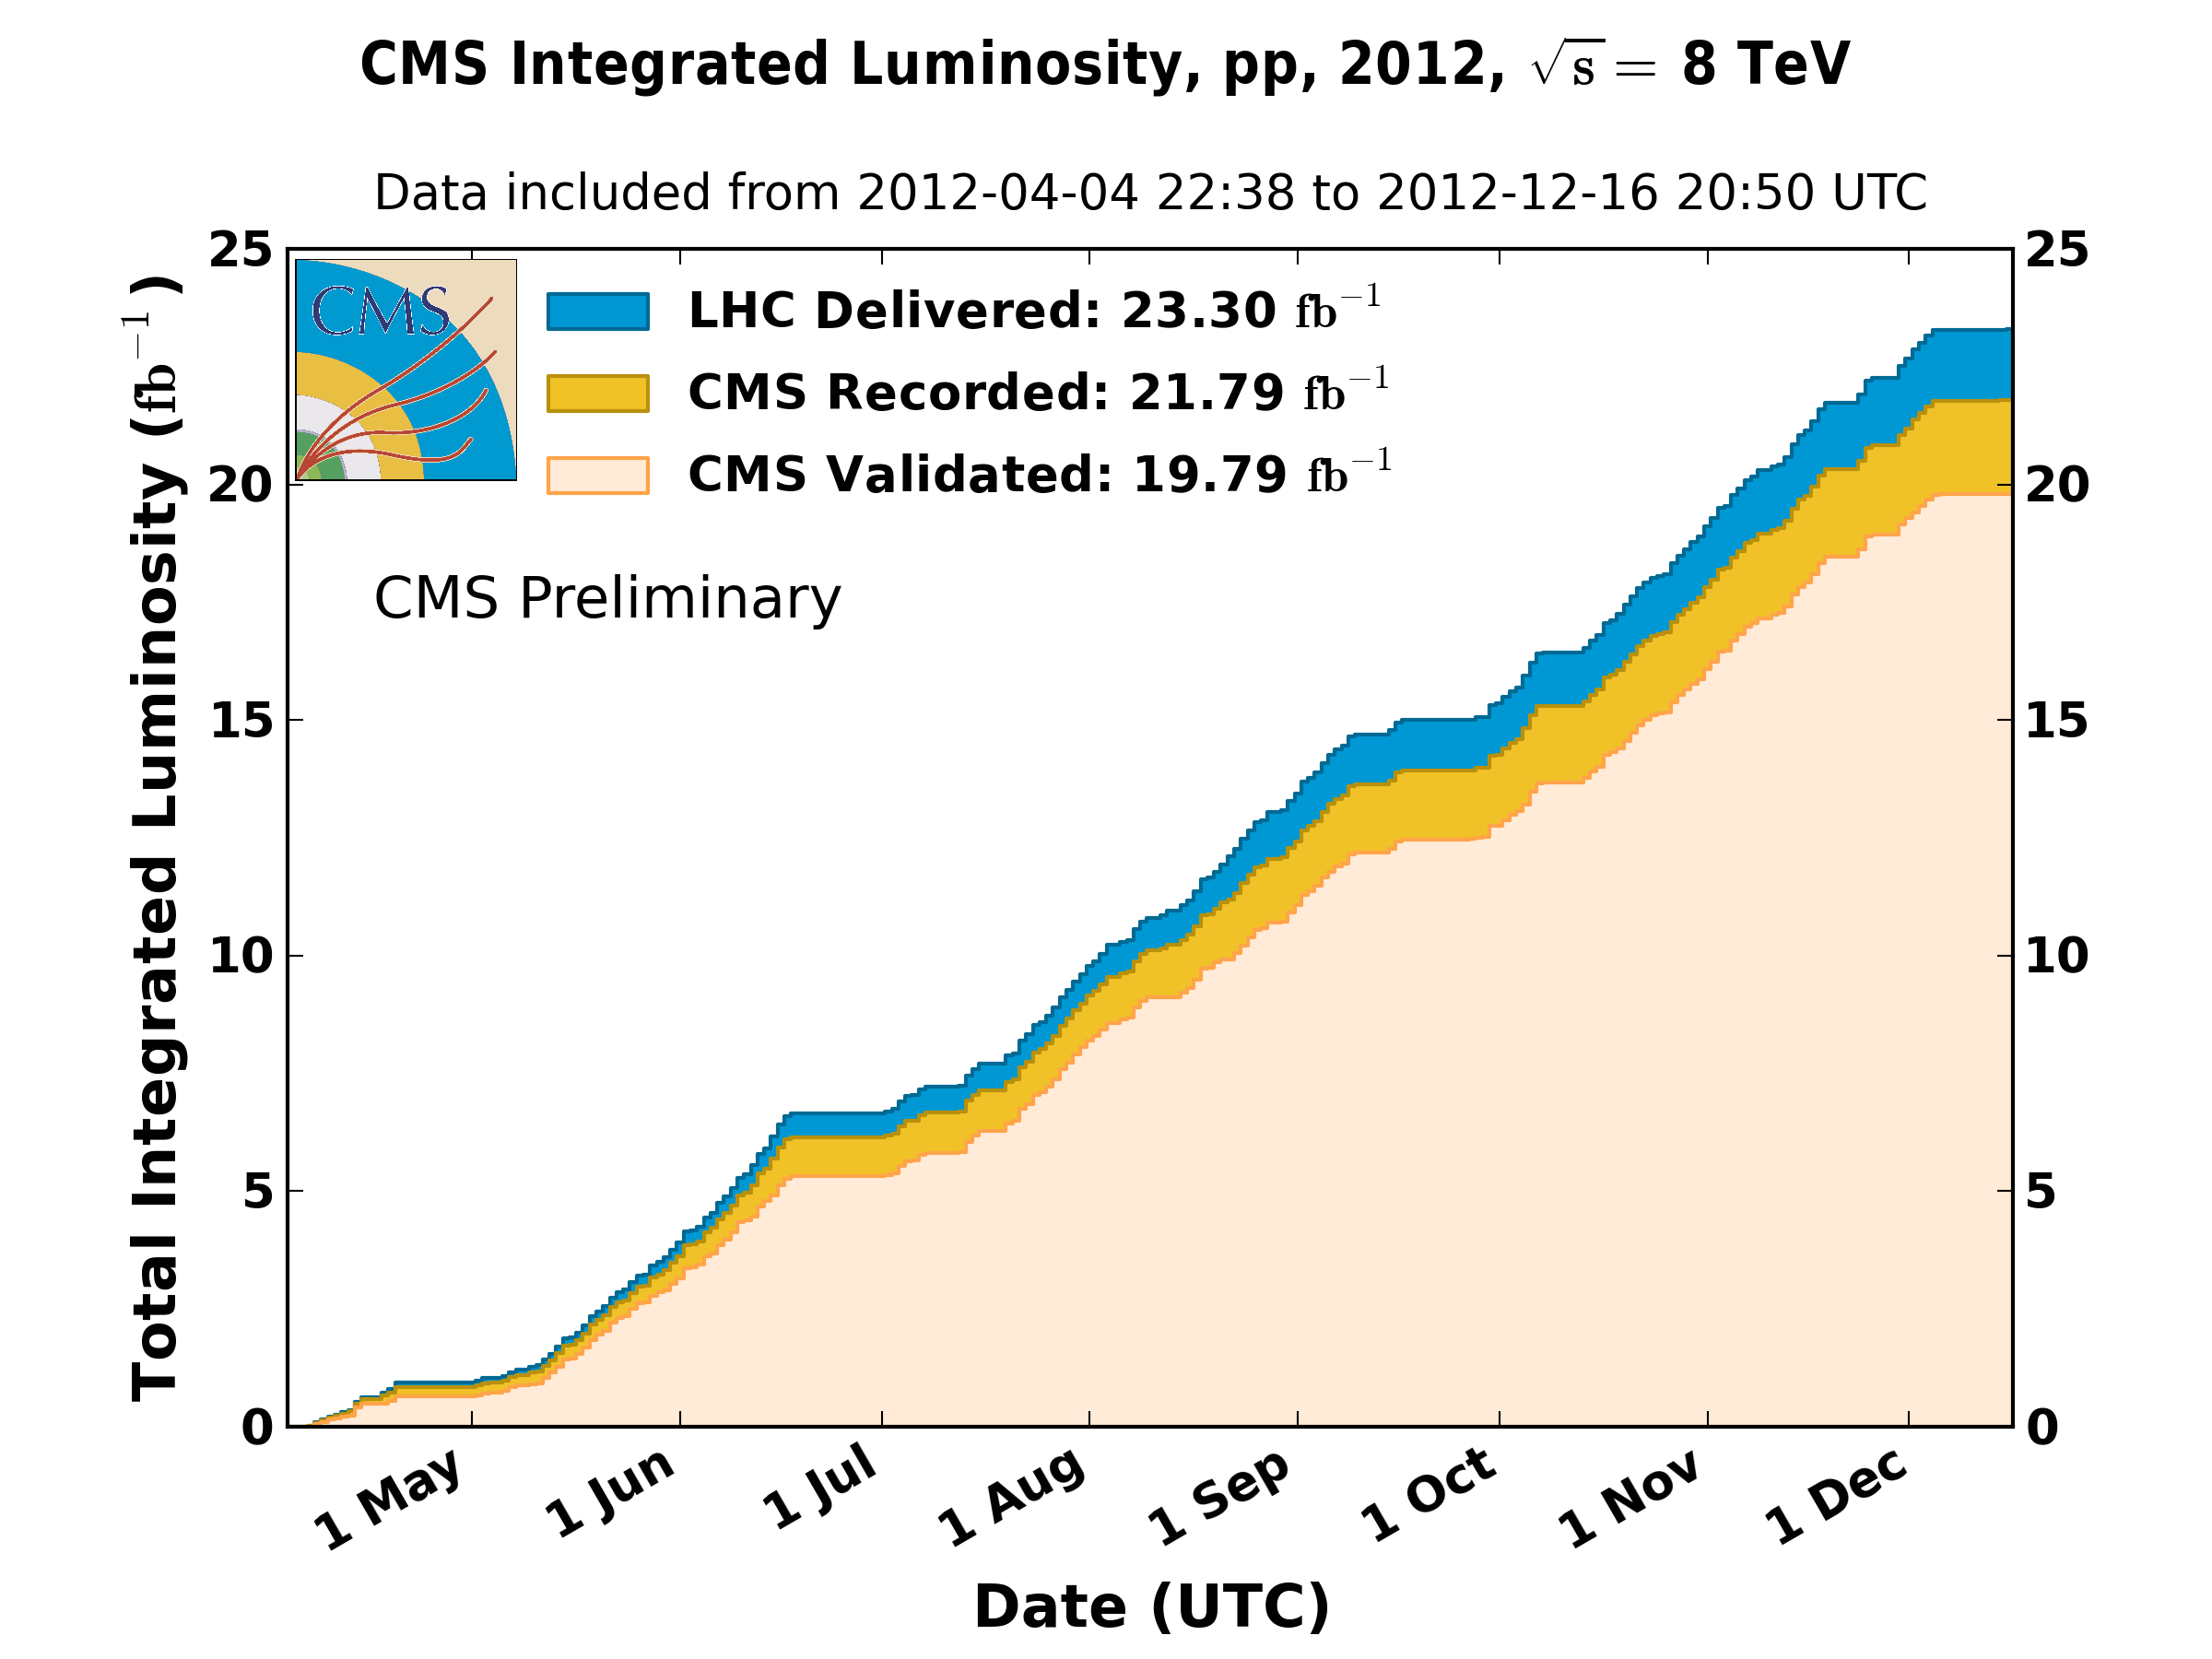
\includegraphics[width=0.95\textwidth]{\figpath/Chapter5/int_lumi_per_day_cumulative_pp_2012_SummerConf.png}
    \caption{Cumulative day-by-day integrated luminosity in 2012 delivered by the LHC (blue), recorded by CMS (dark orange), and validated for physics use (light orange)~\cite{DataQuality}.}
    \label{fig:int_lumi_per_day}
\end{figure}

\begin{table}[hbtp]\footnotesize
\centering
\begin{tabular}{l l l}
\hline
 Dataset & Run Range & Integrated Luminosity \\
\hline
/SingleMu/Run2012A-13Jul2012-v1/AOD & 190645-196531 & 0.809$\fbinv$ \\
/SingleMu/Run2012A-recover-06Aug2012-v1/AOD & 190782-190949 & 0.082$\fbinv$ \\
/SingleMu/Run2012B-13Jul2012-v1/AOD & 193834-196531 & 4.383$\fbinv$ \\
/SingleMu/Run2012C-24Aug2012-v1/AOD & 198022-198523 & 0.489$\fbinv$ \\
/SingleMu/Run2012C-PromptReco-v2/AOD & 194631-203002 & 6.285$\fbinv$ \\
/SingleMu/Run2012D-PromptReco-v1/AOD & 194480-208686 & 7.231$\fbinv$ \\
{\bf Total SingleMu} & {\bf 190645--208686} & {\bf 19.279$\fbinv$} \\
\hline
/SingleElectron/Run2012A-13Jul2012-v1/AOD & 190645-196531 & 0.809$\fbinv$ \\
/SingleElectron/Run2012A-recover-06Aug2012-v1/AOD & 190782-190949 & 0.082$\fbinv$ \\
/SingleElectron/Run2012B-13Jul2012-v1/AOD & 193834-196531 & 4.336$\fbinv$ \\
/SingleElectron/Run2012C-24Aug2012-v1/AOD & 198022-198523 & 0.489$\fbinv$ \\
/SingleElectron/Run2012C-PromptReco-v2/AOD & 194631-203002 & 6.194$\fbinv$ \\
/SingleElectron/Run2012D-PromptReco-v1/AOD & 194480-208686 & 7.238$\fbinv$\\
{\bf Total SingleElectron} & {\bf 190645--208686} & {\bf 19.148$\fbinv$} \\
\hline
\end{tabular}
\caption{The datasets analyzed for this analysis.}
\label{tab:dataSamples}
\end{table}

\subsection{Monte Carlo}

This analysis makes use of MC simulation to study the background processes which have similar final states to that of the \HWWlvjj signal.
Both the kinematic distributions and the final yields are extracted from these samples.
The MC simulation is used for all backgrounds except for the multijet process, where a data-driven approach is used instead.
The process of developing this sample is described in detail in the section~\ref{sec:QCD_data-driven_sample}.
The signal sample kinematics and yields are also taken from MC.
Tables~\ref{tab:SignalSamples} and~\ref{tab:bkgSamples} list all of the MC sample for the Higgs signals and SM background processes, respectively.
The SM background and volunteer signal samples are centrally produced by the CMS collaboration.
The \ggH samples were produced specifically for this analysis.
All of the samples, regardless of who produced them, are stored in a database called the Data Aggregation System (DAS) and organized by the ``Dataset Name'' field.
The backgrounds were modeled by MC samples generated with \textsc{MadGraph}~\cite{Alwall:2014hca} and \textsc{pythia6}~\cite{1126-6708-2006-05-026}. 
The signal MC samples were also generated by \textsc{pythia6}.
Tables~\ref{tab:bkgSamples} and~\ref{tab:SignalSamples} list all of the MC for the Higgs signal and SM background processes, respectively.

\begin{sidewaystable}[hbtp]\footnotesize
\centering
\begin{tabular}{l p{0.50\textwidth} l l}
\hline
\multicolumn{4}{c}{Signal Processes} \\
\hline
Production \& Decay Modes & Dataset Name & Cross Section [\unit{pb}] & BR\\  \hline
\ggH; $\MH=\text{125}\gev$, \HWWlvjj & /LQ-ggh125\_BIG\_SIM\_ggH125\_part1/aperloff-LQ-ggh125\_AODSIM\_Summer12\_START53\_V7E-{\newline}768a14b04b0ac2af0d20e6783fbdb759/USER & 19.27 & 0.0947 \\
  & /LQ-ggh125\_BIG\_GEN\_part2/aperloff-LQ-ggh125\_BIG\_RECO\_part2-33e909ff21293ad9fa8564de2959fe54/USER & 19.27 & 0.0947\\
  & /LQ-ggh125\_BIG\_GEN\_part3/aperloff-LQ-ggh125\_BIG\_RECO\_part3-33e909ff21293ad9fa8564de2959fe54/USER & 19.27 & 0.0947\\
  & /LQ-ggh125\_Part6\_SIM/goodell-LQ-qqh125\_RECO\_Part6-33e909ff21293ad9fa8564de2959fe54/USER & 19.27 & 0.0947\\
  & /LQ-ggh125\_Part7\_SIM/goodell-LQ-qqh125\_RECO\_Part7-33e909ff21293ad9fa8564de2959fe54/USER & 19.27 & 0.0947\\
  & /LQ-ggh125\_Part8\_GENSIM/goodell-LQ-ggh125\_Part8\_RECO-33e909ff21293ad9fa8564de2959fe54/USER & 19.27 & 0.0947\\
\qqH; $\MH=\text{125}\gev$, \HWWlvjj & /LQ-vbf125\_GENSIM/ajkumar-LQ-qqh125\_AODSIM\_Summer12\_{\newline}START53\_V7A-c8f8ed334db8a7d6f56c62266b1dfa5b/USER & 1.578 & 0.0947\\
\WH, \ZH, \ttH; $\MH=\text{125}\gev$, \HWW, inclusive & /WH\_ZH\_TTH\_HToWW\_M-125\_8TeV-pythia6 & 1.249 & 0.215\\\hline
\multicolumn{4}{c}{Non signal Higgs Production} \\ \hline
\WH, \ZH, \ttH; $\MH=\text{125}\gev$, \HZZ, inclusive & /WH\_ZH\_TTH\_HToZZ\_M-125\_8TeV-pythia6 & 1.249 & 0.0264\\
\WH; $\MH=\text{125}\gev$, \Hbb, \Wlv & /WH\_WToLNu\_HToBB\_M-125\_8TeV-powheg-herwigpp & 0.7046 & 0.1879\\
\ttH; $\MH=\text{125}\gev$, \Hbb & /TTH\_HToBB\_M-125\_8TeV-pythia6 & 0.1293 & 0.577\\
\hline
\end{tabular}
\caption{List of signal datasets and cross sections. All of the centrally produced sample names are followed by /Summer12\_DR53X-PU\_S10\_START53\_V7A-v1/AODSIM.}
\label{tab:SignalSamples}
\end{sidewaystable}

\begin{sidewaystable}[hbtp]\footnotesize
\centering
\begin{tabular}{l p{0.65\textwidth} l}
\hline
\multicolumn{3}{c}{Background Processes} \\
\hline
Process & Dataset Name & Cross Section [\unit{pb}] \\
\hline
\Wjets & /WJetsToLNu\_TuneZ2Star\_8TeV-madgraph-tarball & 37509 \\
\ttbar & /TTJets\_MassiveBinDECAY\_TuneZ2star\_8TeV-madgraph-tauola & 225.197 \\
\Zjets & /DYJetsToLL\_M-50\_TuneZ2Star\_8TeV-madgraph-tarball & 3387.6 \\
\WW & /WW\_TuneZ2star\_8TeV\_pythia6\_tauola & 54.838 \\
\WZ & /WZ\_TuneZ2star\_8TeV\_pythia6\_tauola & 33.21 \\
\ZZ & /ZZ\_TuneZ2star\_8TeV\_pythia6\_tauola & 17.654 \\
$\cPqt\rightarrow\cPqb\ell\nu$ (\cPqs-channel) & /T\_s-channel\_TuneZ2star\_8TeV-powheg-tauola & 3.79 \\
$\cPqt\rightarrow\cPqb\ell\nu$ (\cPqt-channel) & /T\_t-channel\_TuneZ2star\_8TeV-powheg-tauola & 56.4 \\
$\cPqt\rightarrow{X}$ (\cPqt\W-channel) & /T\_tW-channel-DR\_TuneZ2star\_8TeV-powheg-tauola & 11.1 \\
$\cPaqt\rightarrow\cPqb\ell\nu$ (\cPqs-channel) & /Tbar\_s-channel\_TuneZ2star\_8TeV-powheg-tauola & 1.76 \\
$\cPaqt\rightarrow\cPqb\ell\nu$ (\cPqt-channel) & /Tbar\_t-channel\_TuneZ2star\_8TeV-powheg-tauola & 30.7 \\
$\cPaqt\rightarrow{X}$ (\cPqt\W-channel) & /Tbar\_tW-channel-DR\_TuneZ2star\_8TeV-powheg-tauola & 11.1 \\
QCD (\Pe-channel) & See table~\ref{tab:dataSamples} for a list of SingleElectron datasets & N/A \\
QCD (\Pmu-channel) & See table~\ref{tab:dataSamples} for a list of SingleMu datasets & N/A \\
\hline
\end{tabular}
\caption{List of background MC datasets and cross sections used in the analysis. Every dataset name is followed by /Summer12\_DR53X-PU\_S10\_START53\_V7A-v1/AODSIM. In addition to v1, this analysis also uses v2 of the \Wjets sample.}
\label{tab:bkgSamples}
\end{sidewaystable}

The \ttbar, \Wjets, and \Zjets SM background samples are generated using \textsc{Mad}\textsc{Graph} v5.1.3.30~\cite{Alwall:2014hca}.
The \ttbar sample is inclusive, meaning that it includes all decay modes of the \W boson coming from the top decay.
The \Wjets and \Zjets samples are also inclusive, but in this case it means that in addition to the leptonic decay of the boson there are any number of final state jets.
The single top quark samples are modeled using the \textsc{POWHEG} 1.0 r138 ~\cite{POWHEG2,POWHEG:singlet,POWHEG:singletW} generator.
The diboson processes use the \textsc{pythia} v6.4.24 generator~\cite{1126-6708-2006-05-026}.
The cross sections for the \ttbar and single top quark processes are calculated at next-to-next-to-leading logarithmic (NNLL) accuracy~\cite{TOPCrossSec} while the inclusive \Wjets and \Zjets processes are calculated at next-to-next-to-leading order (NNLO) accuracy~\cite{FEWZ}.
The diboson cross sections are calculated at next-to-leading order (NLO) accuracy~\cite{MCFM}.

The \HWW signal samples are generated with \textsc{pythia} v6.4.24~\cite{1126-6708-2006-05-026}, where one \W is required to decay leptonically while the other is required to decay hadronically.
The cross sections for the Higgs production are calculated at NNLL QCD and NLO EW accuracies.
The calculations for gluon-gluon fusion and VBF production cross sections use the complex-pole-scheme (CPS) while the associated production cross section are calculated with the zero-width-approximation (ZWA)~\cite{Heinemeyer:2013tqa}.
These samples were privately produced because the centrally produces samples did not include enough events and had large statistical fluctuations.

\subsection{Multijet-QCD Background}
\label{sec:QCD_data-driven_sample}

It is well known that the QCD process is difficult to model to the desired level of accuracy.
Additionally, the event selection in this analysis requires two isolated jets and an isolated lepton, which vastly reduces the number of QCD MC events that pass the selection criteria.
Although the probability to mis-reconstruct a jet as a lepton is fairly low, the production cross section for the multijet process is extremely high and thus cannot be ignored.
When using the MC samples we are left with a statistically limited sample that is almost useless for describing this background.

Rather than relying on MC for the QCD background sample, a data-driven sample was created by using the same trigger requirements as the data, but removing the isolation requirement for the lepton and inverting the lepton particle flow isolation cut during selection.
The main idea of the method is to utilize differences in lepton identification properties that separate prompt, isolated leptons from \W and \Z decays, also known as ``real leptons,'' from non-prompt, non-isolated leptons, also known as ``fake leptons.''
The normal signal selection requires an isolated lepton, without other particles around it, to limit this sort of ``fake lepton,'' but this is exactly the type of property we want to select for when forming a QCD sample from data.
This process provides a completely orthogonal sample of QCD events from data that won't, and shouldn't be used for signal extraction.
Since we make use of the entire 2012 dataset\footnote{The QCD events are scaled slightly to account for failed jobs (missing luminosity) during processing.}, we end up with statistically rich samples containing lots of mis-identified leptons.

A complete description of the event selection will be discussed in section~\ref{ch:event_selection}, but here I will just talk about the isolation requirements.
The loosest lepton PF isolation requirement used to determine the signal region is $\pfiso<0.2$, which is used to veto on ``loose'' or questionable leptons.
The assumption is that any lepton with $\pfiso>0.2$ is a mis-reconstructed lepton coming from QCD.
For electrons we must also turn off the MVA-based identification requirements as they are stringent enough that they won't allow for any fake leptons to pass our selection.
As mentioned before, the electrons must still pass the ``HLT\_Ele27\_WP80\_v*'' electron trigger used for the data containing our signal.
On the other hand, the muon trigger is changed to be ``HLT\_Mu24\_eta2p1\_v*'' to remove the isolation requirement that was included in the trigger used to select for the signal.

In order to gain greater separation from the signal selection to ensure as little non-QCD contamination as possible, we actually use a minimum isolation requirement of $\pfiso>0.3$.
We also put an upper limit on the PF isolation value to keep the sample from having a bias towards high nPV values.
For electrons the upper limit was 0.7 and for muons it was 2.0.
The $1\sigma$ systematic uncertainty bands for electrons (muons) were selected to be $0.2<\pfiso<0.3$ on the low side and $>$0.7 (2.0) for the high side
Fig.~\ref{fig:PFIsolation} shows the pf isolation values contained in the electron multijet and data samples as a function of $\eta$.

\begin{figure}[!hbt]
    \centering
    \begin{subfigure}[t]{0.475\textwidth}
        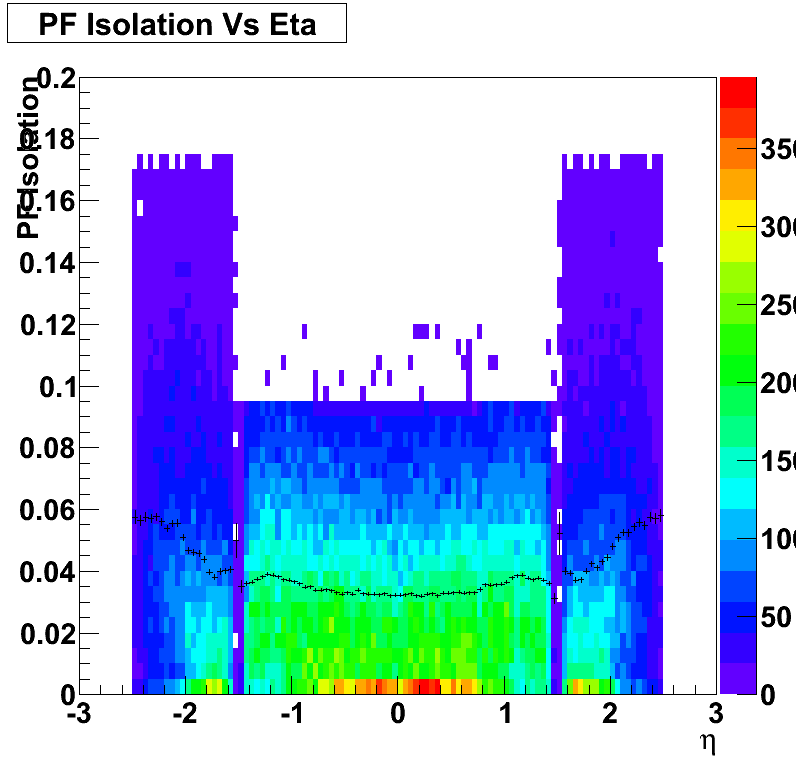
\includegraphics[width=\textwidth]{\figpath/Chapter5/pfIsoVsEta_DATA.png}
        \caption{}
        \label{fig:PFIsolationData}
    \end{subfigure}
    \begin{subfigure}[t]{0.475\textwidth}
        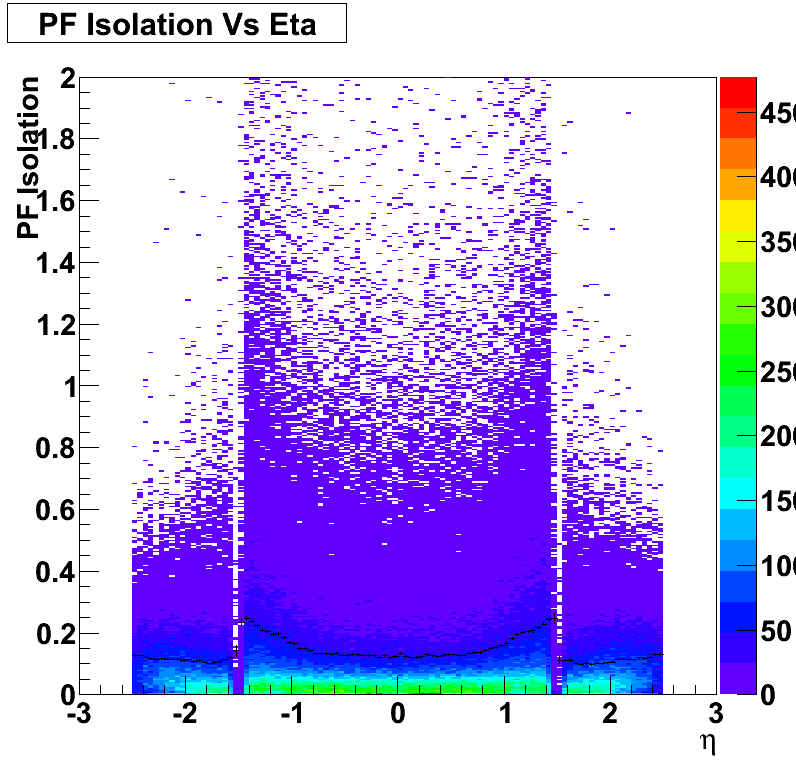
\includegraphics[width=\textwidth]{\figpath/Chapter5/pfIsoVsEta_Full.png}
        \caption{}
        \label{fig:PFIsolationFull}
    \end{subfigure}
    \caption{The PF isolation for the electron channel as a function of $\eta$ (left) with and (right) without the lepton isolation and electron MVA-based identification requirements.}
    \label{fig:PFIsolation}
\end{figure}

\section{Event \& Object Selection}
\label{ch:event_selection}

The reconstruction algorithms described in chapter~\ref{ch:event_reconstruction} are designed to be fairly generic and applicable to a wide array of physics analyses.
Specific groups within CMS called physics object groups (POGs) are responsible for developing object quality criteria which must be implemented by each analysis to prevent fake or poorly reconstructed objects.
This section will discuss the object selection criteria used to identify vertices, electrons, muons, jets, and \VETslash, which all meet or exceed the object requirements as set by the relevant POGs.
Only events which have the right quality and multiplicities of these objects will be used in the analysis.

Like most analyses, this one selects for a single good quality primary vertex, although the presence of additional vertices (pileup) does not disqualify the event.
The primary vertex must pass certain additional quality criteria.
There must be at least four degrees of freedom used to find the vertex, the absolute value of the $z$-coordinate of the vertex must be less than 24\unit{cm}, the absolute value of the $\rho$-coordinate (cylindrical coordinate system) must be less than 2.0\unit{cm}, and the vertex must not be identified as a fake vertex.
These criteria are summarized in table~\ref{tab:vertex_selection}.

\begin{table}[hbtp]\footnotesize
\centering
\begin{tabular}{l l}
\hline
Cut & Value \\
\hline
N\textsubscript{DOF} & $\geqslant$4 \\
$|z|$ & $\leqslant$24\unit{cm} \\
$|\rho|$ & $\leqslant$2.0\unit{cm} \\
\hline
\end{tabular}
\caption{The primary vertex selection requirements for this analysis.}
\label{tab:vertex_selection}
\end{table}

As mentioned before, this analysis selects for the presence of one lepton, either an electron or muon, at least two jets, and some amount of \VETslash.
In practical terms this means that we select for one tight electron (muon) as defined in section~\ref{sec:electrons} (\ref{sec:muons}) and veto the event if there are any additional tight or loose electrons and muons (muons and electrons).
Some additional cuts beyond those of the identification requirements are imposed to cut out some of the background events while maximizing the number of signal events we could use for the multivariate analysis techniques.
The additional \pt and $\eta$ requirements as specified in the same sections are also applied.
For the tight electrons this meant raising the \pt requirement from 27\gev to 30\gev, which avoids using events right on the trigger turn on threshold while only removing $\sim$5\% of signal events, as seen in fig.~\ref{fig:electronPt_signal_loss}. 
Because muon reconstruction and identification in CMS is very good, we only raised the \pt requirement to 25\gev from 24\gev.

\begin{figure}[!hbt]
    \centering
    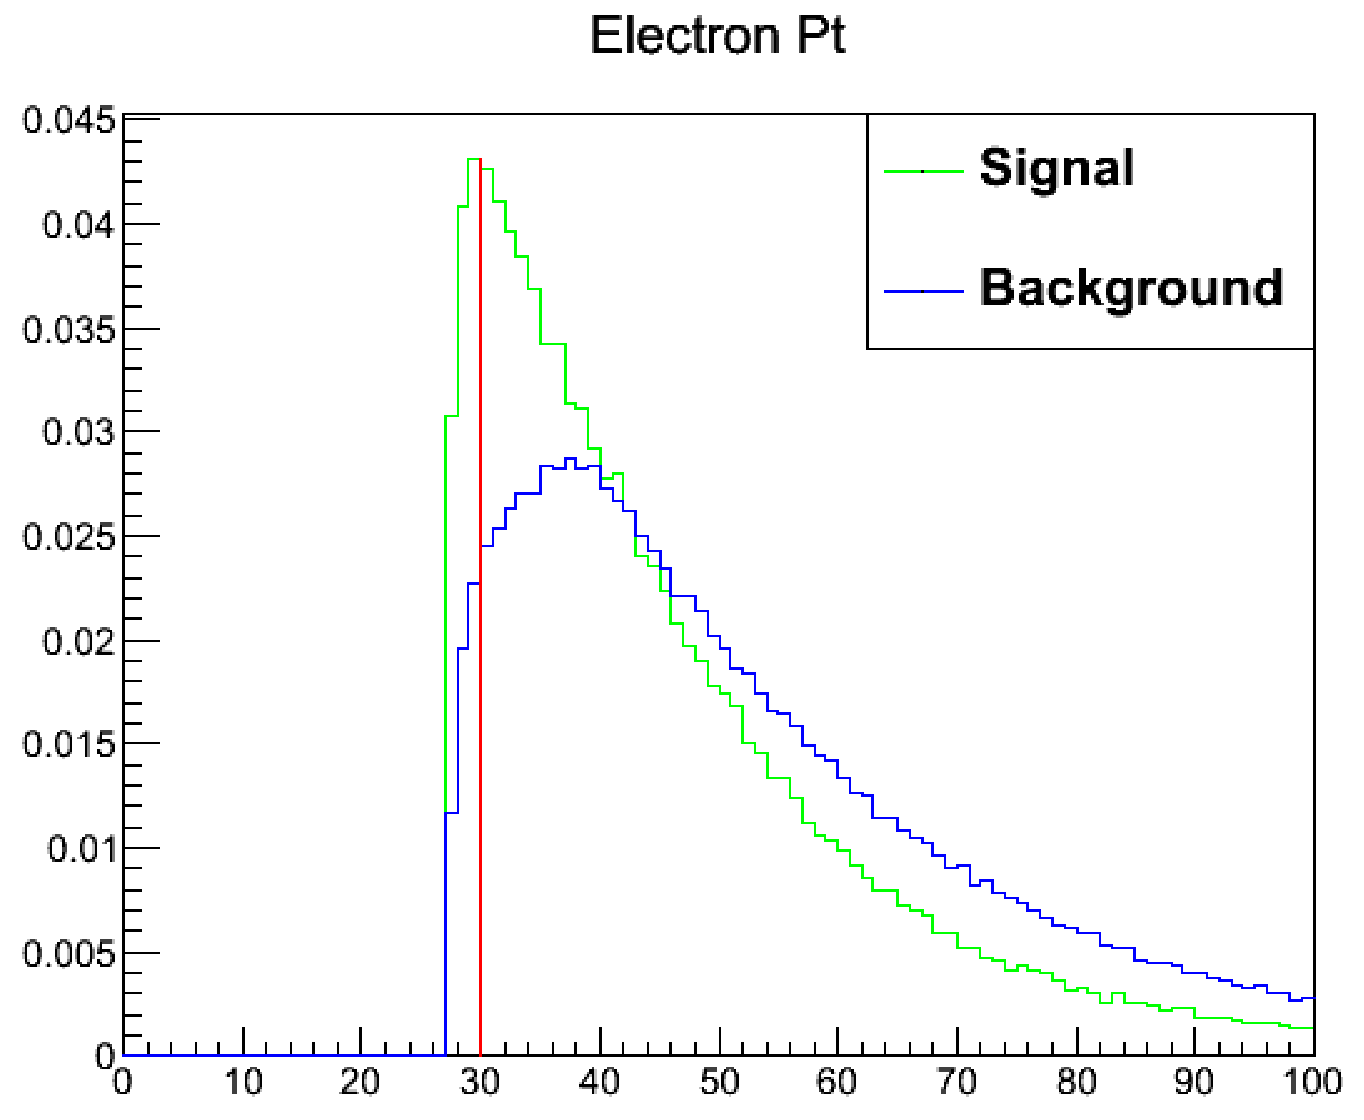
\includegraphics[width=0.95\textwidth]{\figpath/Chapter5/electronPt.png}
    \caption{Histograms of the electron \pt distribution where the gluon-gluon fusion signal is in green and the \Wjets background is in blue. The histograms are normalized to unit area. The red line show the cut on electron \pt where 5\% of the signal is lost.}
    \label{fig:electronPt_signal_loss}
\end{figure}

Beyond the lepton requirements, this analysis selected for any number of jets as long as they pass the selection criteria found in section~\ref{sec:jets}.
As the hadronic W decay will have at least two jets, that is the minimum number of jets needed to make it into the signal region, but we do not veto on additional jets which might come from ISR or FSR.
The requirement of the leading jet having a \ptgt{30}\gev was implemented to reduce the impact of the multijet background while minimally impacting the signal.
Besides the logical splitting of events based on lepton flavor, we also split events into three categories based on the number of jets in the event; exactly two jets, exactly three jets, and four or more jets.
As stated in section~\ref{sec:MET} we also require at least 25\gev of \VETslash.

Given that our signal has only one hadronic \W boson, we don't expect the $\W\rightarrow\bbbar$ branching fraction to contribute much to our signal.
However, we also want to remove as many \ttbar or single top events as possible, which are commonly associated with \cPqb quarks.
Thus we decided to veto events with b-tagged jets in order to reduce our backgrounds as much as possible.
An additional reason to do this is to keep the orthogonality between this analysis and another CMS analysis which was looking at the \VH production channel where \Hbb.
That analysis uses the same final state as this one, but requires two b-tagged jets~\cite{PhysRevD.89.012003}.
To prevent overlap, we only ever considered events with one or fewer b-tagged jets and then we separate the events into two categories based on the number of b-tags.
The zero b-tag events are used for signal extraction while the one b-tag events, which have a much larger impact from \ttbar and a higher \Hbb signal yield, are used for validation purposes and to check the volunteer signal contribution.

%Should I show the cut flow tables for 1-btagged category?

\section{MC Corrections}

Although a significant amount of work and time goes into making sure the MC simulation properly models the data, there can still exist discrepancies between the observed data and simulation
%there are still some corrections which must be made to the reconstructed objects or scale factors which must apply to weight each event in order to accurately mimic the behavior in data.
Often this occurs because the exact data taking conditions are not known in advance, like the pileup conditions that will exist.
Another reason the MC might not exactly mimic the data is that even state of the are generators are limited in their precision; much of the physics of hadronization is still unknown and hard physics processes can often only be computed up to NLO precision.
Data, on the other hand, contains all hadronization effects and all orders of precision.
I have already discussed some object specific corrections like the jet energy corrections, jet energy resolution, and \VETslash corrections in sections~\ref{sec:jets} and~\ref{sec:MET}.
For other discrepancies it is often necessary to reweight the full event rather than a specific object.

Broadly speaking these corrections can be separated into two categories: those which are common to all CMS analyses and those which are specific to this analysis.
The first category includes the b-tagging CSV discriminant weights and top quark \pt spectrum weights for the \ttbar simulation while the second category includes the weights for our multijet sample.
These event weights are applied after selecting for the events as they do not change the object kinematics.

\subsection{Pileup Reweighting}

Pileup is an important quantity as it can affect the reconstruction efficiency and even the observed kinematics of all the objects used in this analysis.
Up to this point it has been described as additional proton-proton interactions within an event, besides the interaction that produced the physics objects we are interested in studying.
There are several other properties of pileup which are worth noting.
I have so far either referred to pileup in a general sense or as relating to additional objects (tracks or energy) which might be found in the same bunch crossing as the event under study.
In reality there are two different categories of pileup.
There is indeed the pileup which comes from additional proton-proton interactions within the same bunch crossing, known as ``in-time'' pileup.
There is also energy from pileup added to objects because it was left in the sub-detectors from bunch crossings before or after the current one.
This is known as ``out-of-time'' pileup and comes about because the integration window of the sub-detectors can be larger than 25\unit{ns}.
An additional property is somewhat obvious in that the true number of proton-proton interaction within an event, $\mu$, is related to the instantaneous luminosity, which can vary over the course of data taking and even within a luminosity section (LS) period.
As a benchmark, the average number of proton-proton interactions per bunch crossing in 2012 was 21~\cite{LumiPublic}.

\begin{figure}[!hbt]
    \centering
    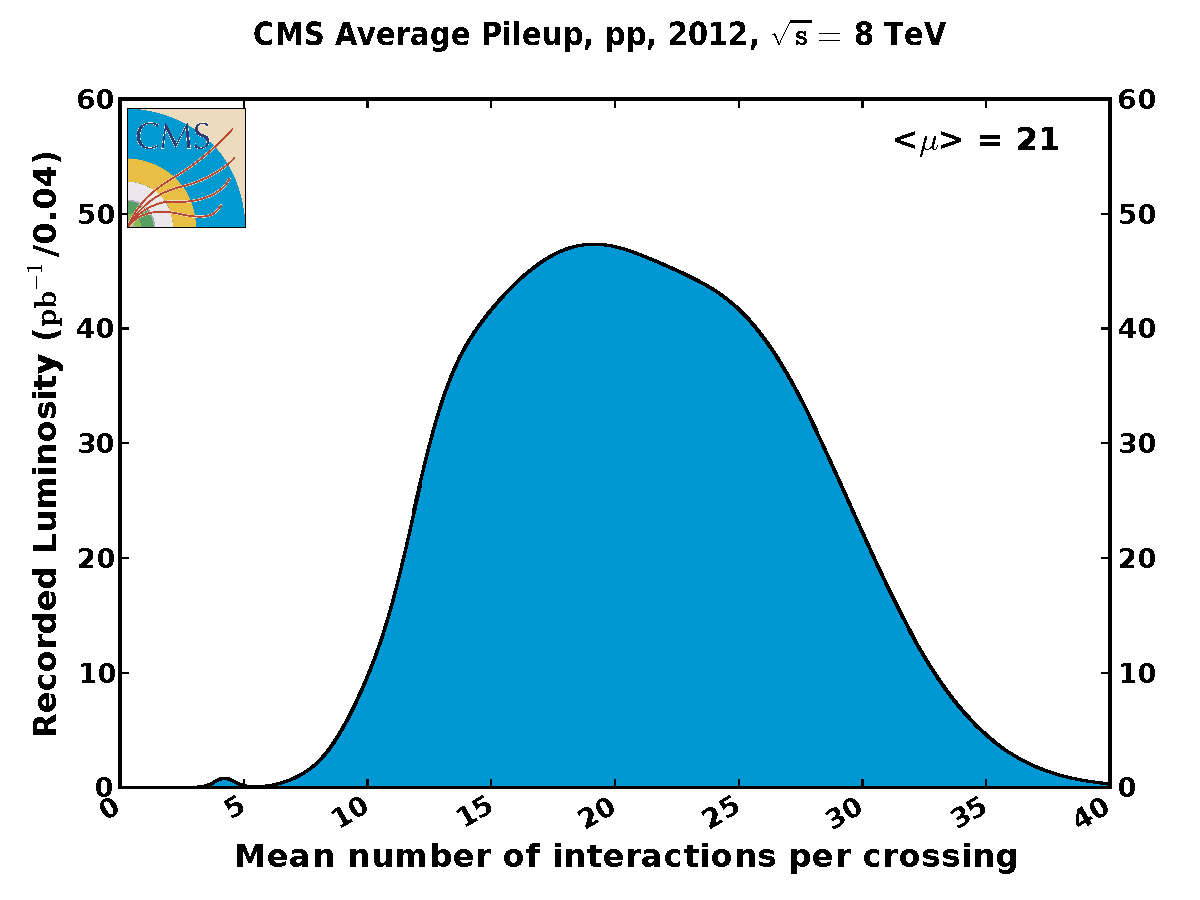
\includegraphics[width=0.95\textwidth]{\figpath/Chapter5/pileup_pp_2012.pdf}
    \caption{The mean number of interactions per bunch crossing in 2012. The min-bias cross section used for the calculation is 80\unit{mb}.}
    \label{fig:pileup_pp_2012}
\end{figure}

The MC samples used in CMS are usually generated before the data is taken and are thus created with an assumption of what the pileup conditions will look like in data.
A broad distribution of $\mu$ values, the number of min-bias pileup events overlaid on the hard scatter event, is generally chosen so as to cover all pileup conditions which might be experienced over the course of a data taking period.
Somewhat unsurprisingly the anticipated $\mu$ distribution rarely matches the one one observed in the data and thus the MC must be reweighted such that the $\mu$ distributions match~\cite{PileupStudiesTwiki}.
To generate a histogram for the average number of interactions per bunch crossing coming from data we make use of the approved pileupCalc tool provided by CMS.
This tool takes as input the total inelastic cross section $\sigma_{\text{inelastic}}=69.3\unit{mb}$\footnote{This is the CMS approved best fit value, not the theoretical value.}, a file in JSON format with every run number and luminosity section matched to a given average instantaneous luminosity and integrated luminosity for that given LS, and another JSON formatted file with the run numbers and LS used in the given analysis\footnote{This analysis uses the full 2012 ``golden'' JSON file called\\Cert\_190456-208686\_8TeV\_PromptReco\_Collisions12\_JSON.txt.}.
All of the MC samples used contain the same $\mu$ distribution scenario denoted by the ``S10'' notation in the dataset name.
The per event weights as a function of $\mu$ are created by dividing the normalized distribution from data by the normalized MC based distribution.
The weights are then applied to each MC event by looking up the weight for the mean number of pileup interactions used to generate that specific event~\cite{PileupWeightTwiki}. The distributions of pileup interactions in MC and data a well as the corresponding pileup weights can be seen in fig.~\ref{fig:pileup_reweighting}. Unfortunately, because the weights are not at unity, the statistical precision of the MC samples is reduced.
Fig.~\ref{fig:npv_comparison} shows the data to MC comparison of the N\textsubscript{PV} distribution before and after the pileup reweighting scheme has been applied.

\begin{figure}[!hbt]
    \centering
    \begin{subfigure}[t]{0.48\textwidth}
      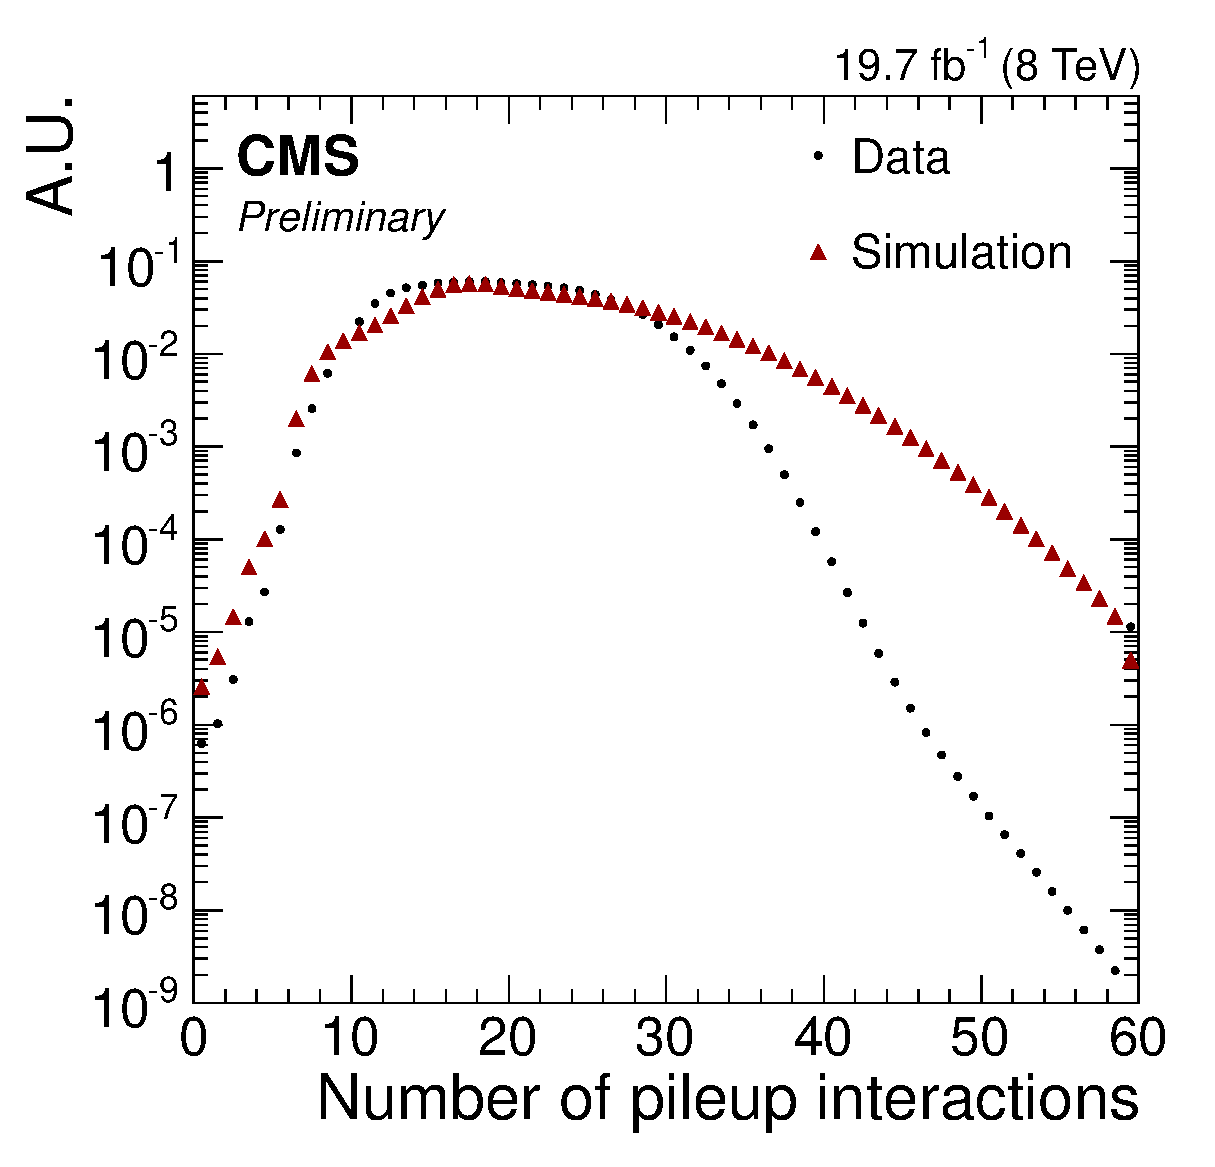
\includegraphics[width=0.95\textwidth]{\figpath/Chapter5/PileupDistribution.eps}
      \caption{}
      \label{fig:tnpu_distributions}
    \end{subfigure}
    \begin{subfigure}[t]{0.48\textwidth}
      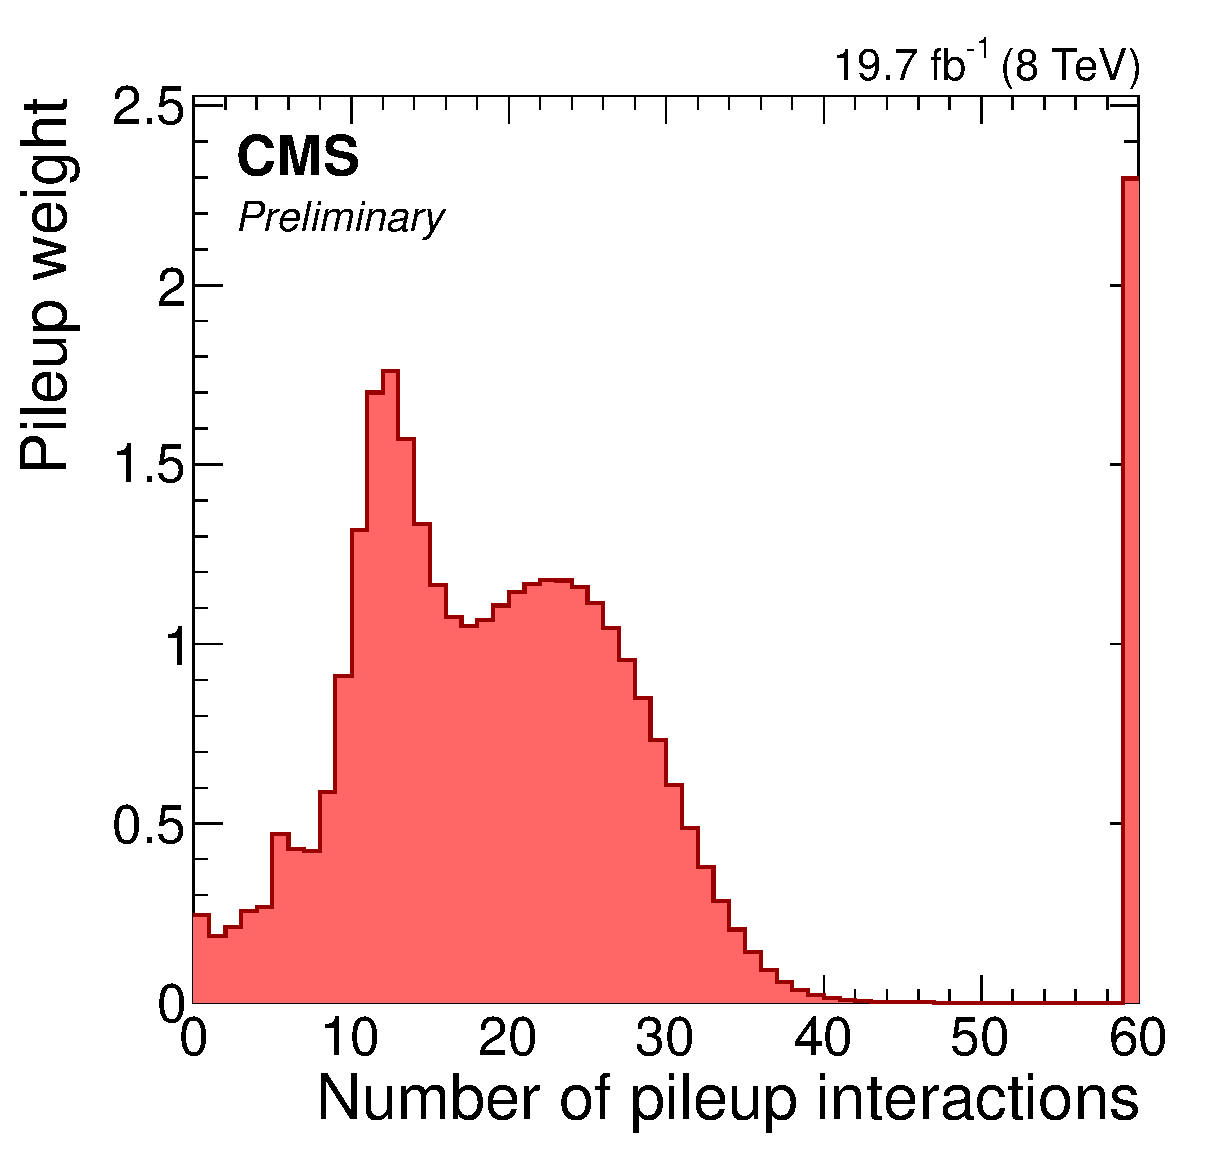
\includegraphics[width=0.95\textwidth]{\figpath/Chapter5/PileupWeights.eps}
      \caption{}
      \label{fig:pileup_weights}
    \end{subfigure}
    \caption{(a) Distributions of the number of pileup interactions in data and in simulation. (b) The derived pileup weights as a function of the number of interactions.}
    \label{fig:pileup_reweighting}
\end{figure}

\begin{figure}[!hbt]
    \centering
    \begin{subfigure}[t]{0.48\textwidth}
      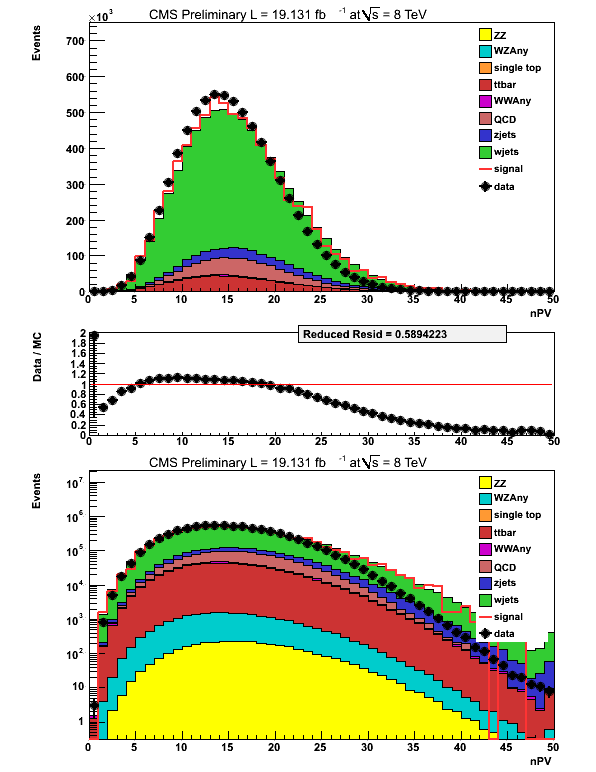
\includegraphics[width=\textwidth]{\figpath/Chapter5/nPV_noRW__comblep.png}
      \caption{}
      \label{fig:npv_no_pileup_reweight}
    \end{subfigure}
    \begin{subfigure}[t]{0.48\textwidth}
      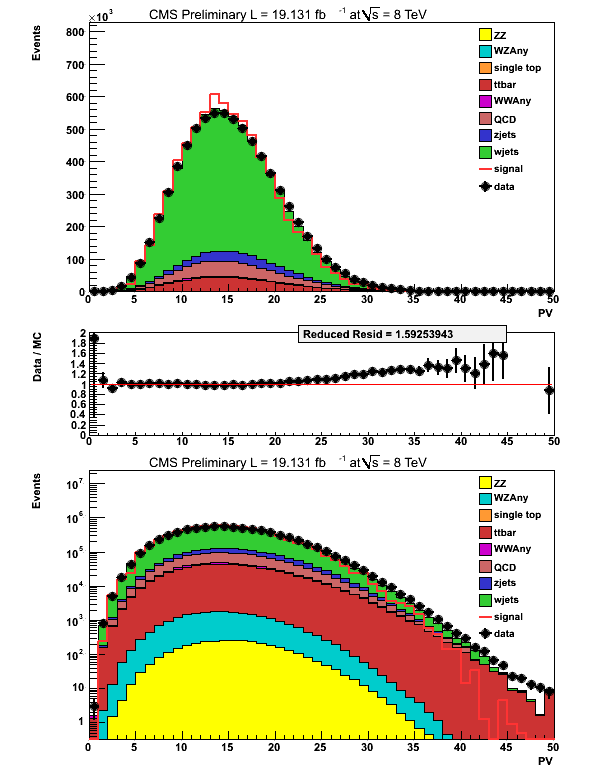
\includegraphics[width=\textwidth]{\figpath/Chapter5/nPV__comblep.png}
      \caption{}
      \label{fig:npv_pileup_reweight}
    \end{subfigure}
    \caption{Comparison of the number of primary vertices (N\textsubscript{PV}) in data and in MC (a) before the the pileup weights are applied and (b) after the weights are applied. These distributions correspond to the 19\fbinv collected during the 2012 data taking period and include both the electron and muon categories.}
    \label{fig:npv_comparison}
\end{figure}

While this methodology is sufficient for the simulated backgrounds, it does not work for the data-driven multijet background.
As can be seen from figs.~\ref{fig:QCDvData_nPV_ele} and~\ref{fig:QCDvData_nPV_mu}, the distributions for the number of primary vertices between data and the QCD samples do not match, indicating some bias due to the selection.
Since the QCD sample does not contain the truth level number of pileup interactions, this is data after all, it would be improper to look up pileup weights using the same weight distribution as for simulation.
Instead, a new set of weights is derived using the number of primary vertices for data in the signal region and anti-isolated region, assuming that the vertex finding efficiency is the same in both regions and only the selection of the lepton changes.
These weights can be seen in figs.~\ref{fig:QCD_PUWeights_ele} and~\ref{fig:QCD_PUWeights_mu} and are applied in the same manner as before.

\begin{figure}[!hbt]
    \centering
    \begin{subfigure}[t]{0.48\textwidth}
        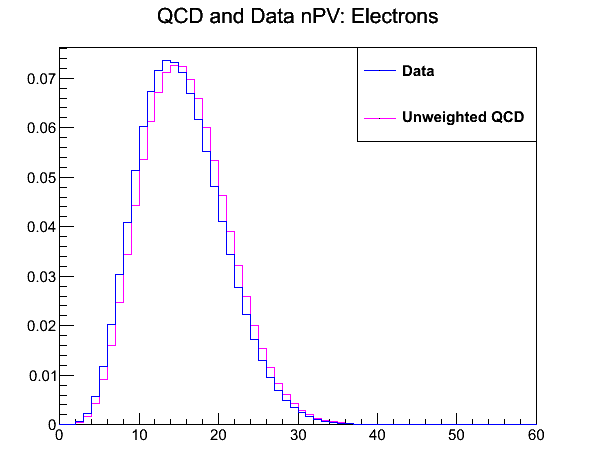
\includegraphics[width=\textwidth]{\figpath/Chapter5/QCD_PUWeights/QCDvData_nPV_ele.png}
        \caption{}
        \label{fig:QCDvData_nPV_ele}
    \end{subfigure}
    \begin{subfigure}[t]{0.48\textwidth}
        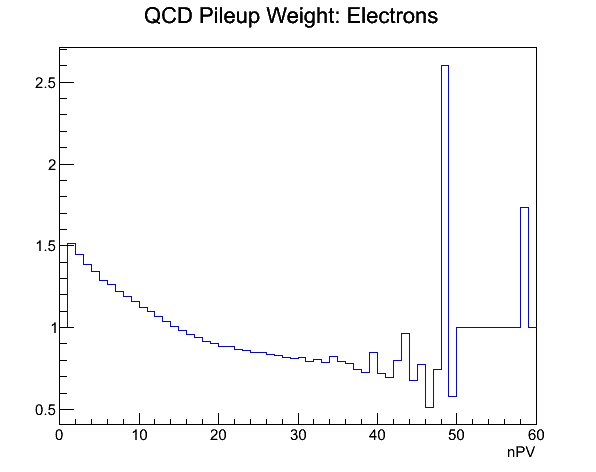
\includegraphics[width=\textwidth]{\figpath/Chapter5/QCD_PUWeights/QCD_PUWeights_fromTree_ele.png}
        \caption{}
        \label{fig:QCD_PUWeights_ele}
    \end{subfigure}

    \begin{subfigure}[t]{0.48\textwidth}
        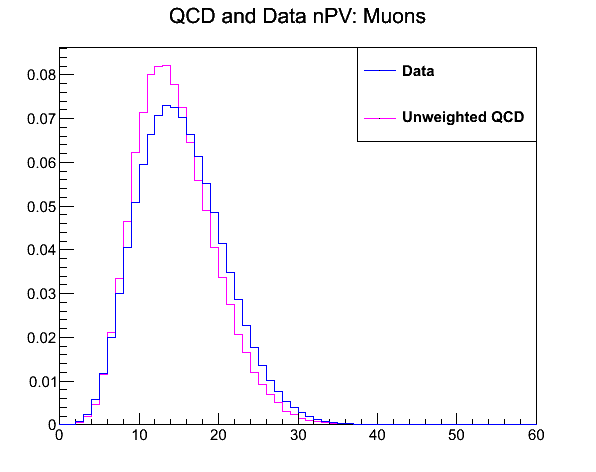
\includegraphics[width=\textwidth]{\figpath/Chapter5/QCD_PUWeights/QCDvData_nPV_mu.png}
        \caption{}
        \label{fig:QCDvData_nPV_mu}
    \end{subfigure}
    \begin{subfigure}[t]{0.48\textwidth}
        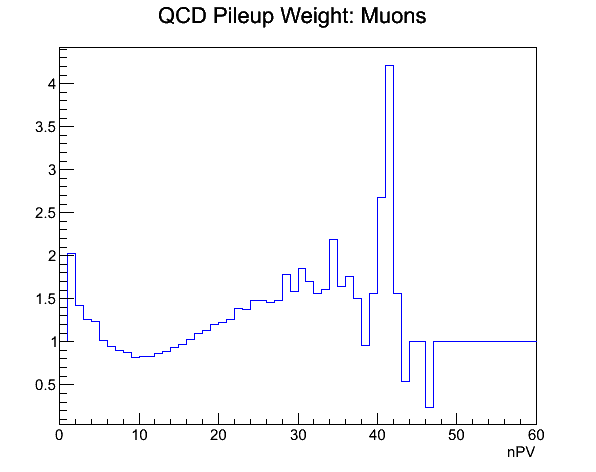
\includegraphics[width=\textwidth]{\figpath/Chapter5/QCD_PUWeights/QCD_PUWeights_fromTree_mu.png}
        \caption{}
        \label{fig:QCD_PUWeights_mu}
    \end{subfigure}
    \caption{Distribution of the number of primary vertices for data and QCD (a,c) and the associated weights (b,c). Figures (a) and (b) show the electron channel while figures (c) and (d) show the muon channel.}
    \label{fig:QCD_PUReweight}
\end{figure}

\subsection{CSV Reweighting}
Section~\ref{sec:btagging} introduced the criterion for tagging a jet as being produced by a \cPqb quark and the use of the Combined Secondary Vertex (CSV) discriminant.
The derivation of this discriminant is described in~\cite{Weiser:927399,BTV-12-001}.
This analysis relies heavily on the identification of \cPqb jets to veto the \ttbar background, so it is absolutely crucial that it behave the same in both data and MC and accurately describe the rate of observing a \cPqb jet.
\cite{CMS-AN-13-130} notes that the tagging efficiency in data is not the same as that in MC, so a correction to the CSV discriminant must be made.
The corrections described there both correct the rate of observing a jet in MC with a CSV value above a given threshold as well as the general shape of the CSV distribution.
If at the end of the procedure the shape of the data and MC distributions agree, then they will also properly assess the rate of events passing a given CSV threshold.

The method is based on calculating a scale factor for both heavy and light flavor quarks which is parameterized by the CSV value, jet \pt, and, in the case of light flavor quarks, jet $\eta$.
We first retrieve the truth level jet flavor in order to determine the correct category: \cPqb jet, \cPqc jet, or light flavor (anything else).
The \cPqc jets are given a flat scale factor of 1, meaning that there is no need to correct the CSV value for this flavor.
The \cPqb jet scale factors are divided into five \pt bins of \ptlt{40\gev}, \ptrange{40\gev}{60\gev}, \ptrange{60\gev}{100\gev}, \ptrange{100\gev}{160\gev}, and \ptgt{160\gev}.
The light flavor scale factors are divided into only three \pt bins of \ptlt{40\gev}, \ptrange{40\gev}{60\gev}, and \ptgt{60\gev}, but are also divided into three eta bins of \absetalt{0.8}, \absetaleqlt{0.8}{1.6}, and \absetaleqlt{1.6}{2.4}.
An individual scale factor is retrieved for each jet, which is then combined as in equation~\ref{eq:CSVWeight_SF_total} in order to create an event weight.
\begin{equation}\label{eq:CSVWeight_SF_total}
  SF_{\mathrm{total}}=\prod_{i}^{N_{\mathrm{jets}}}SF_{\mathrm{jet}_{i}}=SF_{\mathrm{jet}_{1}}{\cdot}SF_{\mathrm{jet}_{2}}{\cdot}...
\end{equation}
The CSV value for each jet is unchanged, but the event is weighted by $SF_{\mathrm{total}}$.

\subsection{\texorpdfstring{\ttbar}{TTbar} Reweighting}
Differential top-quark-pair analyses have shown that the shape of the \pt spectrum for top quarks is softer in data than predicted by simulation~\cite{Chatrchyan:2012saa,TopPtReweighting}.
Although it has been shown that NNLO predictions show reasonable agreement~\cite{Kidonakis2014}, this analysis must correct for the discrepancy in the \ttbar simulation.
Events are reweighted based on the \pt of the generator level \cPqt and \cPaqt in only the \ttbar simulation.
The weight $w_{\mathrm{TopPt}}$ is calculated as:
\begin{align}
  w_{\mathrm{TopPt}} ={}& \sqrt{SF_{\cPqt}{\cdot}SF_{\cPaqt}} \label{eq:TopPtWeight} \\
  SF\left(\ptsup{gen}\right) ={}& \exp\left(a+b\ptsup{gen}\right) \label{eq:TopPtSF}
\end{align}
with $a=0.156$ and $b=-0.00141$.
Fig.~\ref{fig:top_pt_weights} shows the distribution of weights for electron and muon events separately.
The bulk of the weights are centered around 1, indicating that no correction is necessary, with a long low side tail, indicating that a good fraction of events require the top \pt to be scaled down.
Some events do require that the top \pt be increased.

\begin{figure}[!hbt]
    \centering
    \begin{subfigure}[t]{0.48\textwidth}
      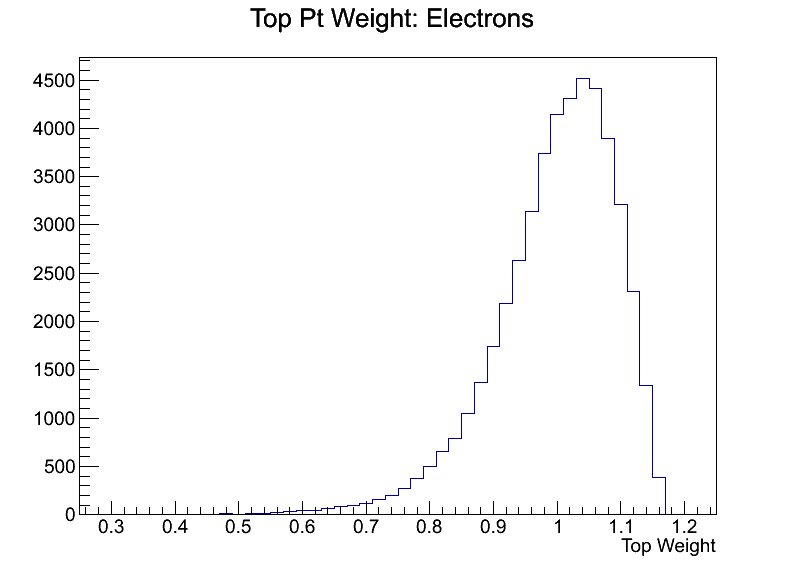
\includegraphics[width=\textwidth]{\figpath/Chapter5/top_weight_ele.png}
      \caption{}
      \label{fig:top_pt_weights_ele}
    \end{subfigure}
    \begin{subfigure}[t]{0.48\textwidth}
      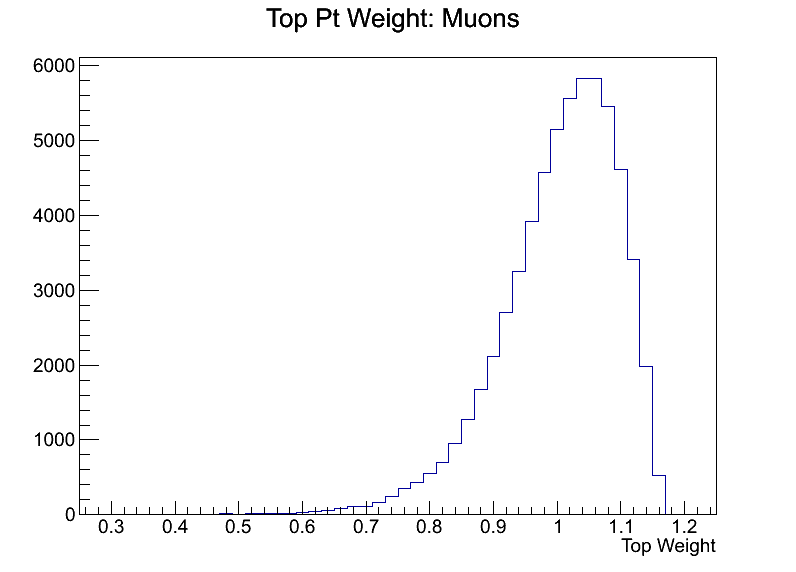
\includegraphics[width=\textwidth]{\figpath/Chapter5/top_weight_mu.png}
      \caption{}
      \label{fig:top_pt_weights_mu}
    \end{subfigure}
    \caption{Top \pt weight distributions for (a) electrons events and (b) muon events.}
    \label{fig:top_pt_weights}
\end{figure}

\subsection{\texorpdfstring{cos(theta$_l$)}{CosThetaL} Reweighting}

A linear trend in the data to MC comparison of the \costhetal variable was discovered, indicating a mis-modeling problem in the simulation.
\costhetal is one of the angular variables involved in the \WW system and is the cosine of the angle between the daughter lepton and the \WW decay plane, which corresponds to $\cos\left(\theta_{2}\right)$ in fig.~\ref{fig:XWWDecayAngles}.
Fig.~\ref{fig:cos_theta_l_preweight_signal} shows this trend in the two jet bin, though the trend is the same in the other jet bins.

\begin{figure}[!hbt]
    \centering
    \begin{subfigure}[t]{0.48\textwidth}
      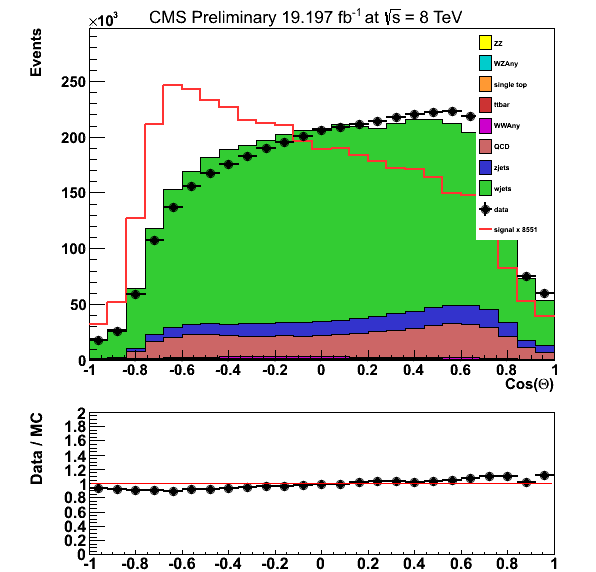
\includegraphics[width=\textwidth]{\figpath/Chapter5/CosThetaPlots/CosThetaL_2Jets_preWeight.png}
      \caption{}
      \label{fig:cos_theta_l_preweight_signal}
    \end{subfigure}
    \begin{subfigure}[t]{0.48\textwidth}
      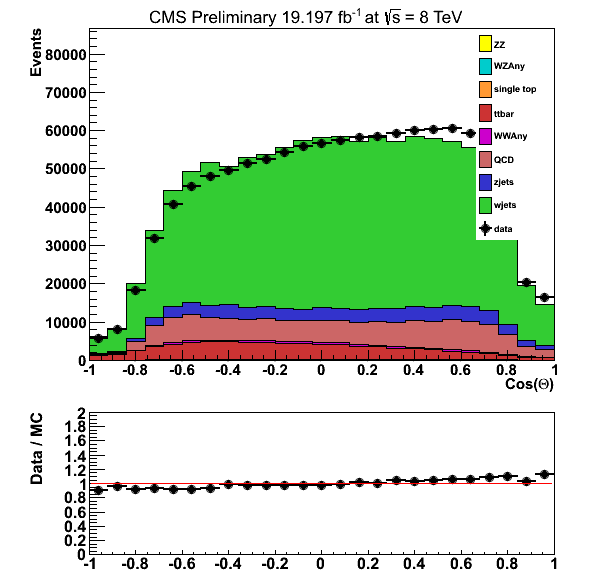
\includegraphics[width=\textwidth]{\figpath/Chapter5/CosThetaPlots/CosThetaL_2Jets_BTagRegion.png}
      \caption{}
      \label{fig:cos_theta_l_preweight_1btag}
    \end{subfigure}
    \caption{Distribution of \costhetal for data and MC in the two jet bin for (a) the signal region and (b) the one b-tag region. The top of each figure shows the data and MC expectations while the bottom shows their ratio with a clear linear trend.}
    \label{fig:cos_theta_l_preweight}
\end{figure}

We correct for the trend in the \Wjets MC as this is the biggest background and correcting it will improve the overall agreement.
We create the corrections in the one b-tag control region shown in fig.~\ref{fig:cos_theta_l_preweight_1btag} so as to not bias our backgrounds in the signal region.
It's clear from fig.~\ref{fig:cos_theta_l_preweight} that the trend in the one b-tag region is the same as the trend in the signal region.
Although the regions are similar, the \ttbar MC plays a much larger role in the control region because it contains two real \cPqb jets.
Therefore we subtract the expected \ttbar yield from the data before creating the weights.
The new weights shown in fig.~\ref{fig:cos_theta_l_weight} are combined multiplicatively with the pileup and CSV weights for the \Wjets sample.
The corrected distribution is shown in fig.~\ref{fig:cos_theta_l_corrected} where it is clear that the trend has been removed.

\begin{figure}[!hbt]
    \centering
    \begin{subfigure}[t]{0.48\textwidth}
      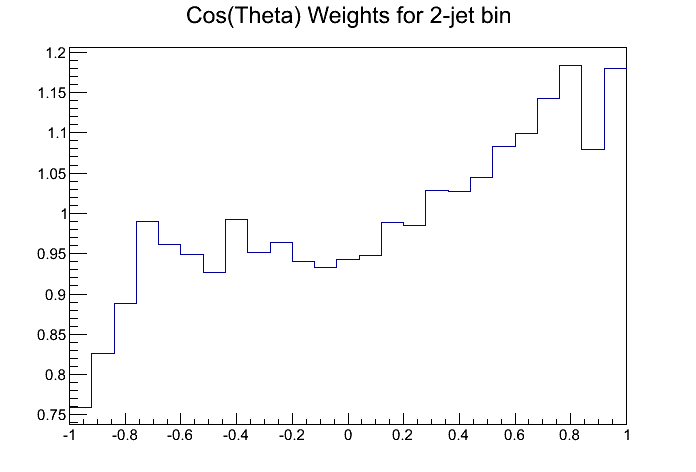
\includegraphics[width=\textwidth]{\figpath/Chapter5/CosThetaPlots/CosThetaWeight_2Jets_lep_ControlRegion.png}
      \caption{}
      \label{fig:cos_theta_l_weight}
    \end{subfigure}
    \begin{subfigure}[t]{0.48\textwidth}
      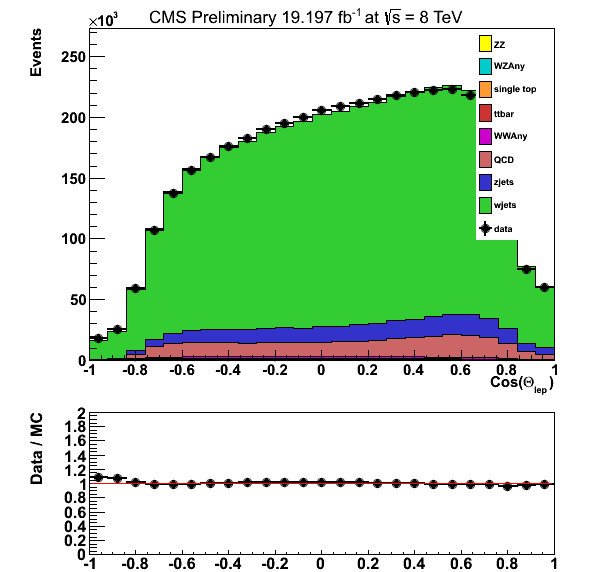
\includegraphics[width=\textwidth]{\figpath/Chapter5/CosThetaPlots/CosThetaL_2Jets_Corrected.png}
      \caption{}
      \label{fig:cos_theta_l_corrected}
    \end{subfigure}
    \caption{(a) Weights created in the one b-tag control region used to correct the \costhetal mis-modeling. (b) \costhetal distribution in the signal region after applying the weights.}
    \label{fig:cos_theta_l_postweight}
\end{figure}

\subsection{QCD Reweighting}

As stated in section~\ref{sec:QCD_data-driven_sample}, the QCD sample is obtained by selecting on anti-isolated leptons, as opposed to the isolated signal selection.
Although these regions are similar kinematically, the ratio of the number of events in the signal region to the number of events in the anti-isolated region changes significantly as a function of $\eta$.
This effect was first noticed in MC, which was used to check the anti-isolation procedure despite its limited statistics in the low \pthat-binned samples.
Fig.~\ref{fig:SfVsEtaMC} shows the suspect ratio as a function of $\eta$ in the different QCD \pthat bins.
The effect seems to be particularly large in the endcap regions (\absetagt{1.3}).
A weighting procedure is necessary to make sure that the expected yield as a function of $\eta$ for the data-driven QCD sample is correct when used in the signal region.

\begin{figure}[!hbt]
    \centering
    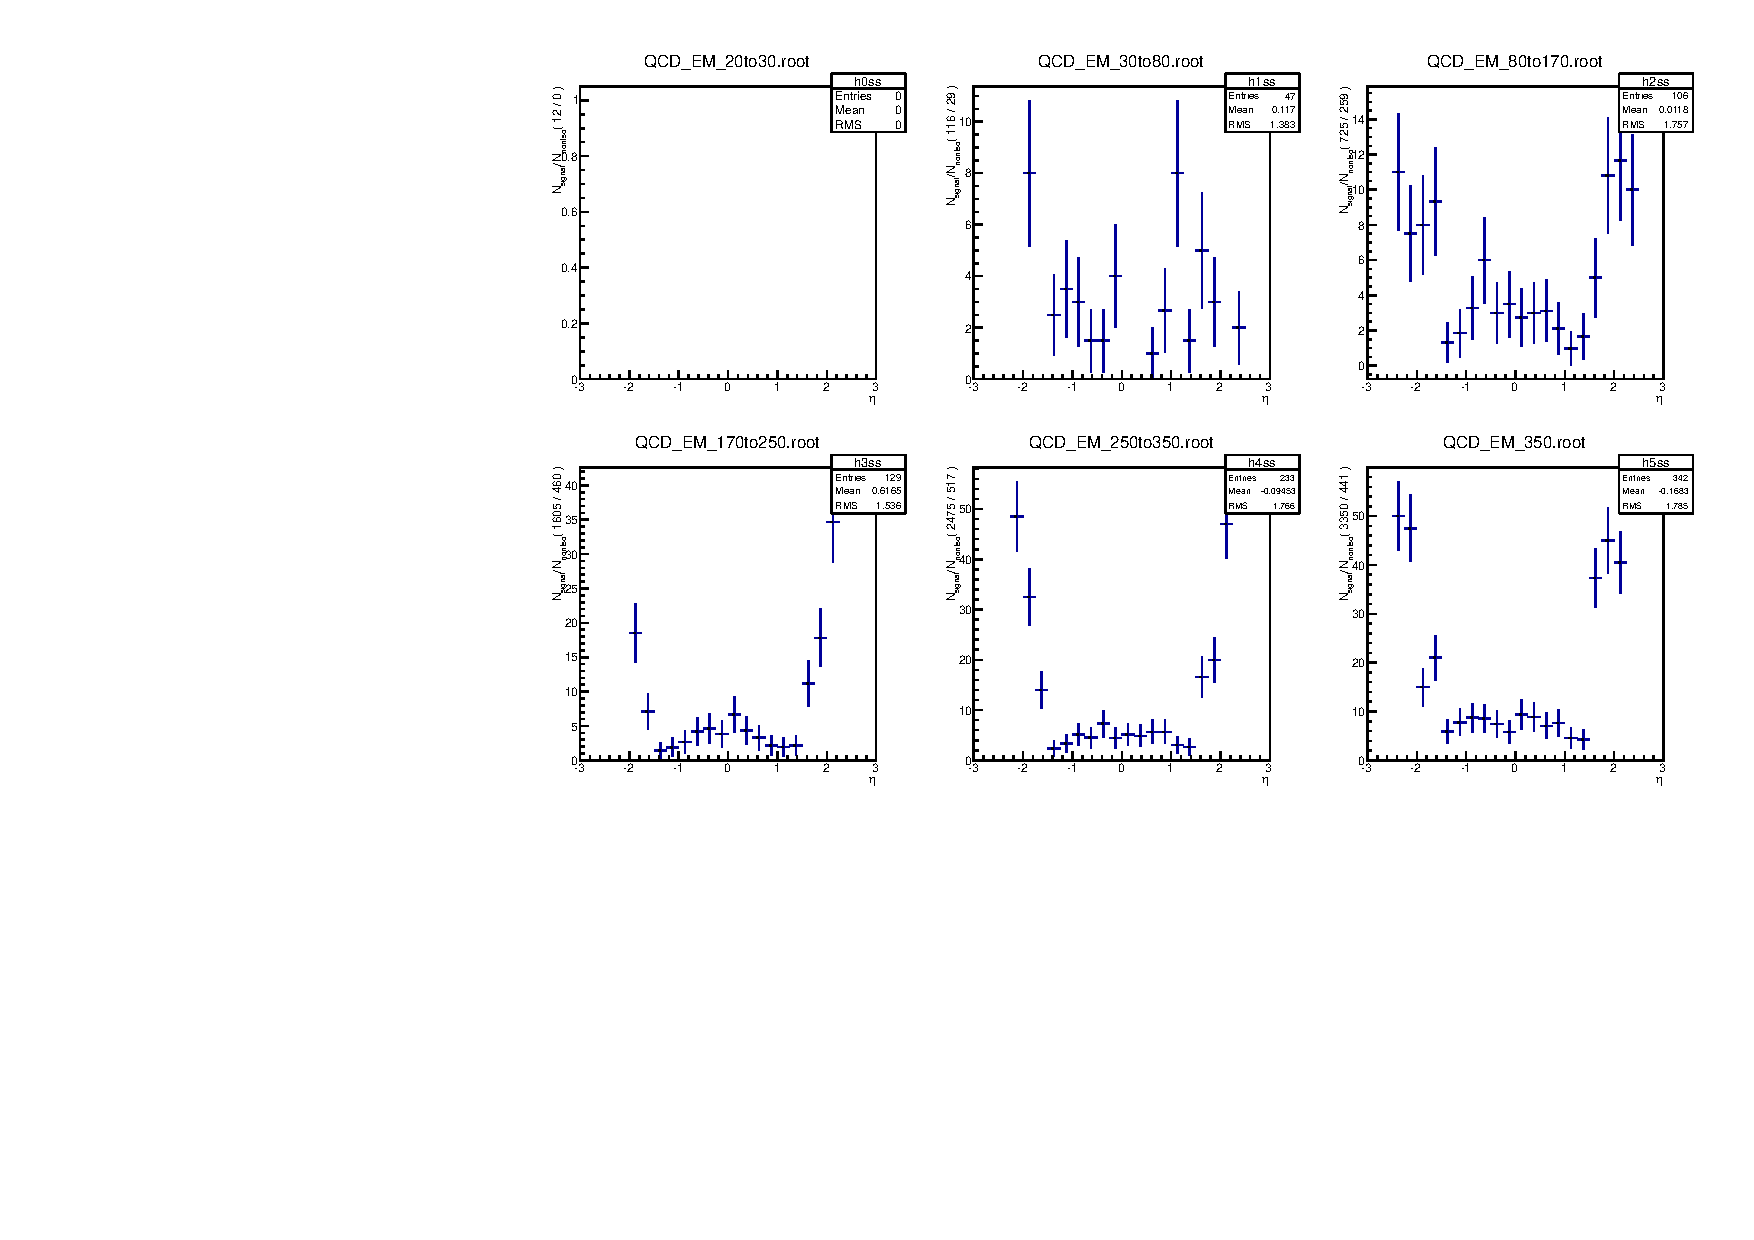
\includegraphics[width=\textwidth]{\figpath/Chapter5/QCD_EtaWeights/SfVsEtaMC.pdf}
    \caption{The ratio of the number of events in the signal region to the number of events in the anti-isolated region for six QCD \pthat bins. The total number of events in the two regions is shown in parentheses along the $y$-axis. The first plot is empty due to the low number of MC events which pass the selection criteria.}
    \label{fig:SfVsEtaMC}
\end{figure}

To derive the weights we use the one jet control region separated into 13 (12) bins of lepton $|eta|$ for the electron (muon) channel.
We want to find the scale factor $S_{\mathrm{QCD}}$ such that:
\begin{equation}
  N_{\mathrm{anti-isolated}}^{\mathrm{QCD}}\left(\eta\right)S_{\mathrm{QCD}}\left(\eta\right)=N_{\text{signal region}}^{\mathrm{QCD}}\left(\eta\right),
\end{equation}
where $N_{\mathrm{anti-isolated}}^{\mathrm{QCD}}$ and $N_{\text{signal region}}^{\mathrm{QCD}}$ represent the number of events in the anti-isolated and signal regions, respectively, given the same luminosity in both.
In order to determine the scale factor needed to to modify the QCD contribution in each bin, we perform a fit to the data using the \ETslash distribution.
The QCD and \Wjets contributions are allowed to float while the contributions from all of the other backgrounds are fixed to their SM expectations.
The \ETslash distributions post-fitting as well as the $\chi^{2}/NDF$ for all of the fits are shown in fig.~\ref{fig:AllMetFits_control6_electron}.
The fit returns both the scale factor $S_{\mathrm{QCD}}$ as well as a scale factor for the \Wjets, $S_{\Wjets}$, which are shown in fig.~\ref{fig:SfVsEta_control6_electron}.
The shape of the weights follows very closely the shape of the ratio in MC from fig.~\ref{fig:SfVsEtaMC}, which is a very good indication that we are indeed correcting for the intended effect.
The same procedure is performed for the muon events, yielding the weights shown in fig.~\ref{fig:SfVsEta_control6_muon}.
Note that the absolute value of the scale factors is not what matters, only their relative values, as the sample will undergo an additional normalization in order to obtain the correct yield.

\begin{figure}[!hbt]
    \centering
    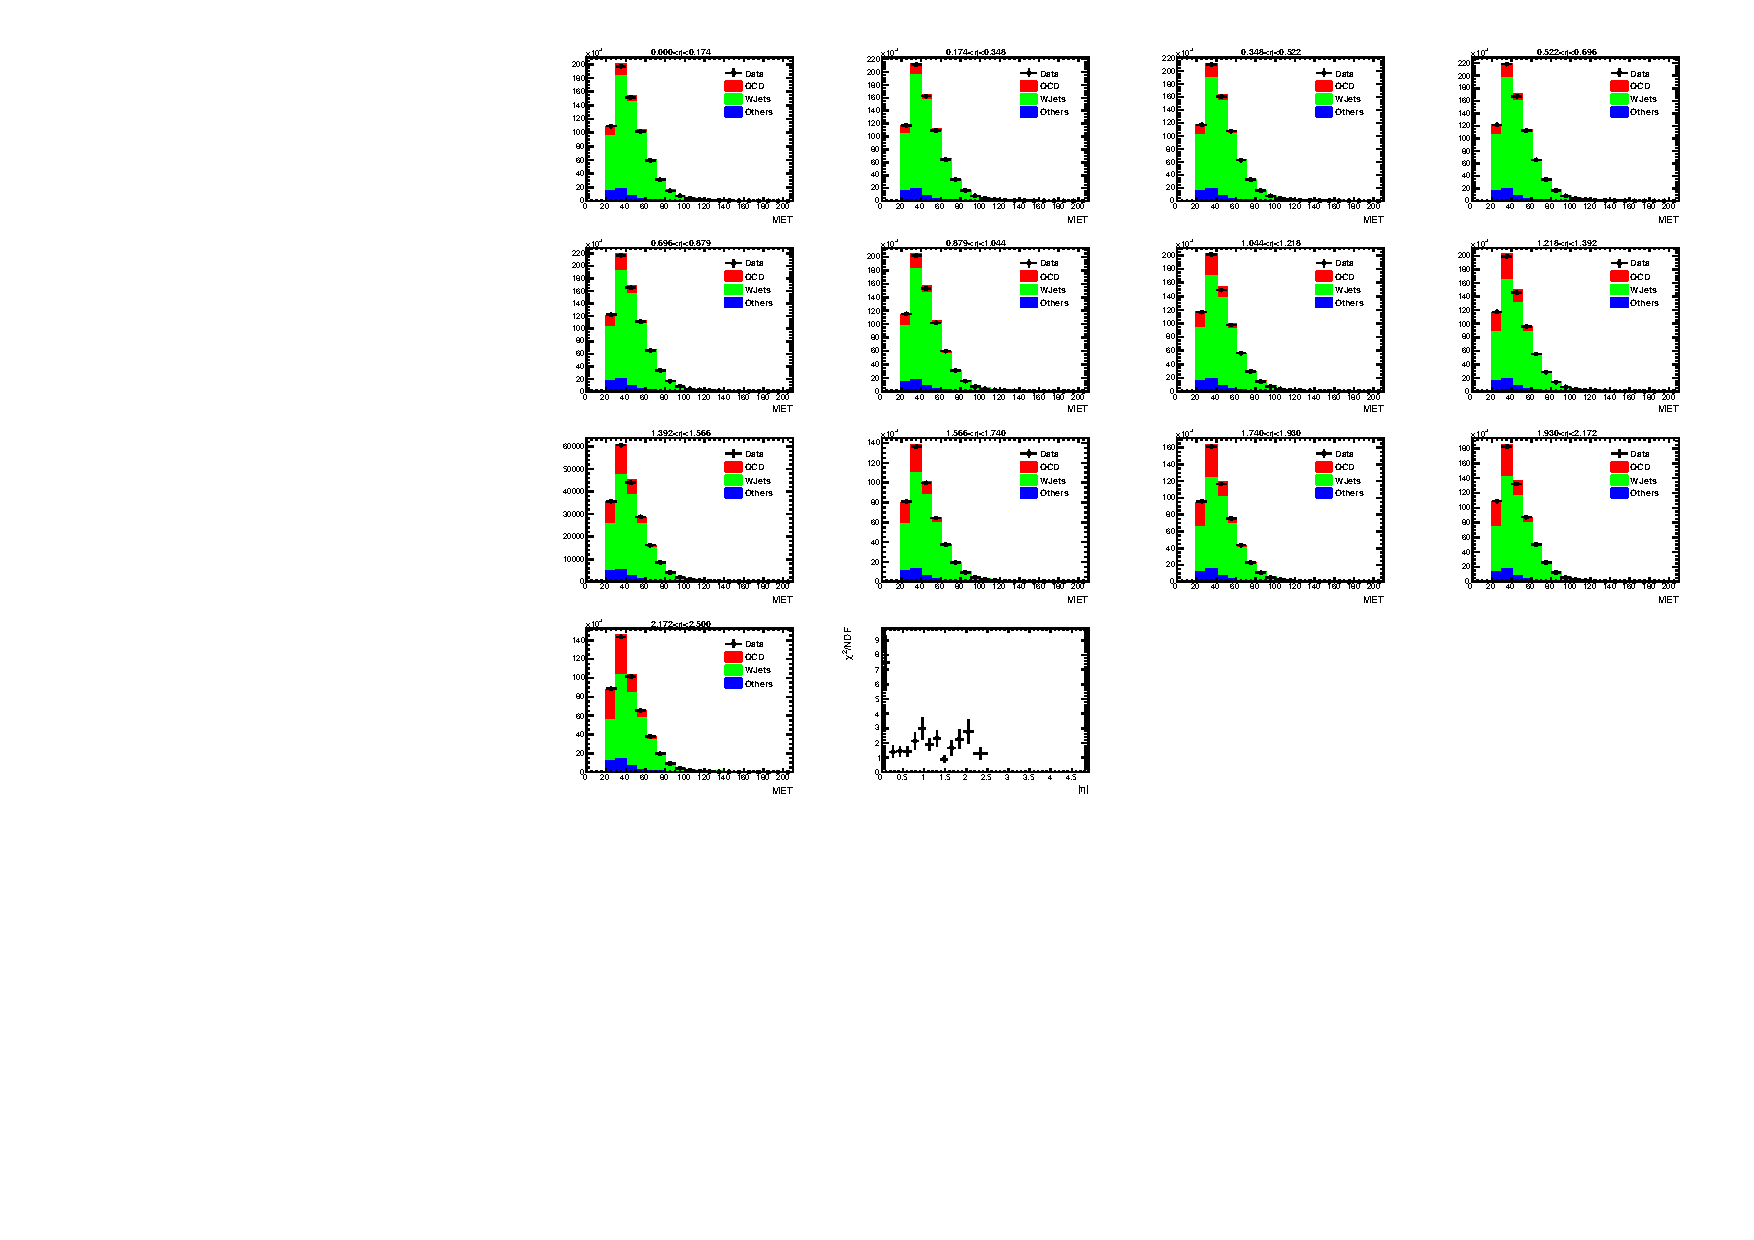
\includegraphics[width=\textwidth]{\figpath/Chapter5/QCD_EtaWeights/AllMetFits_control6_electron.pdf}
    \caption{The \ETslash distributions used to derive the QCD weights in the 13 different bins of lepton $|\eta|$ after the fitting the QCD (red) and \Wjets (green) contributions to the data (black markers). The contribution from the other SM processes (blue) is held fixed to their SM expectation. The last pad in the plot show the $\chi^{2}/NDF$ of the fits.}
    \label{fig:AllMetFits_control6_electron}
\end{figure}

\begin{figure}[!hbt]
    \centering
    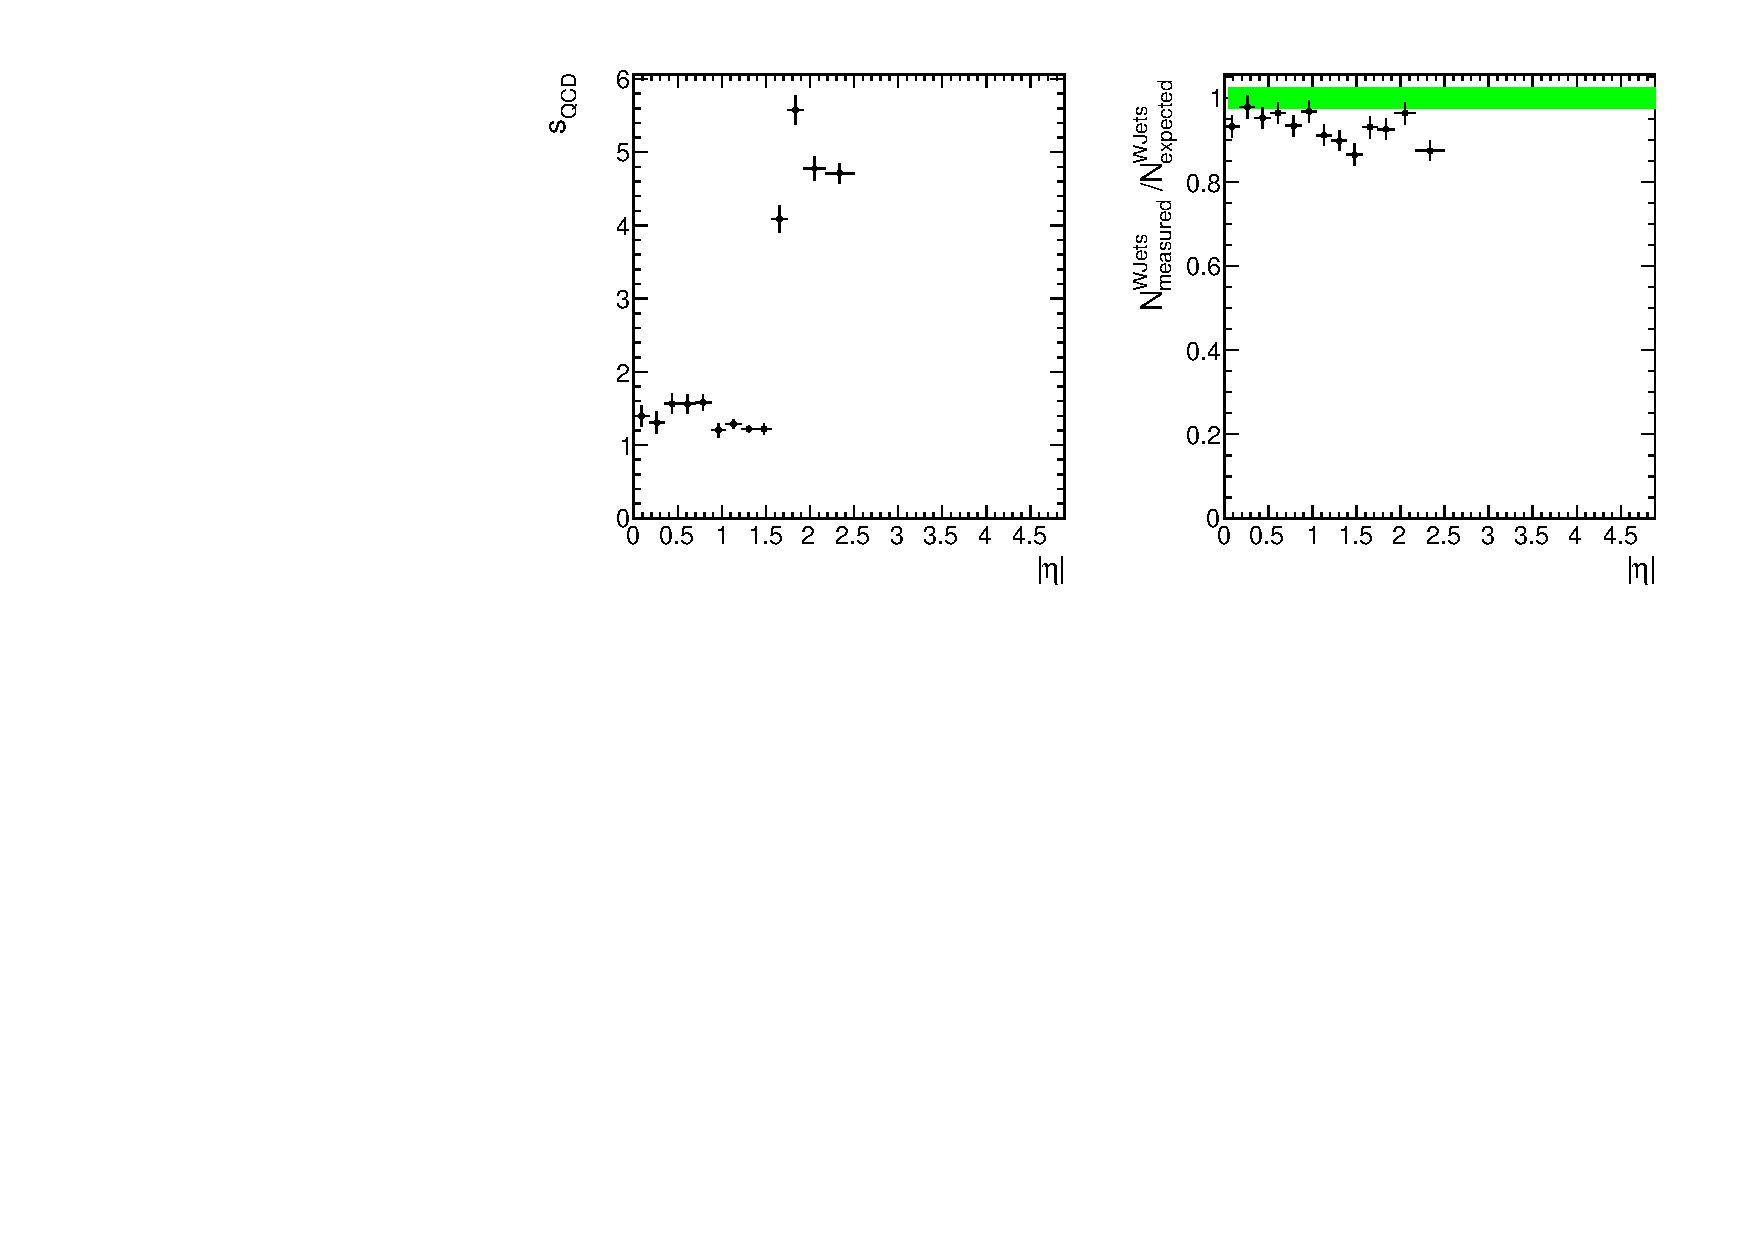
\includegraphics[width=\textwidth]{\figpath/Chapter5/QCD_EtaWeights/SfVsEta_control6_electron.pdf}
    \caption{$S_{\mathrm{QCD}}$ (left) and $S_{\Wjets}$ (right) scale factors as a function of lepton $|\eta|$ derived in the electron channel for the one jet bin. The green band indicates the uncertainty on the \Wjets expectation due to the theoretical uncertainty in the SM cross section.}
    \label{fig:SfVsEta_control6_electron}
\end{figure}

\begin{figure}[!hbt]
    \centering
    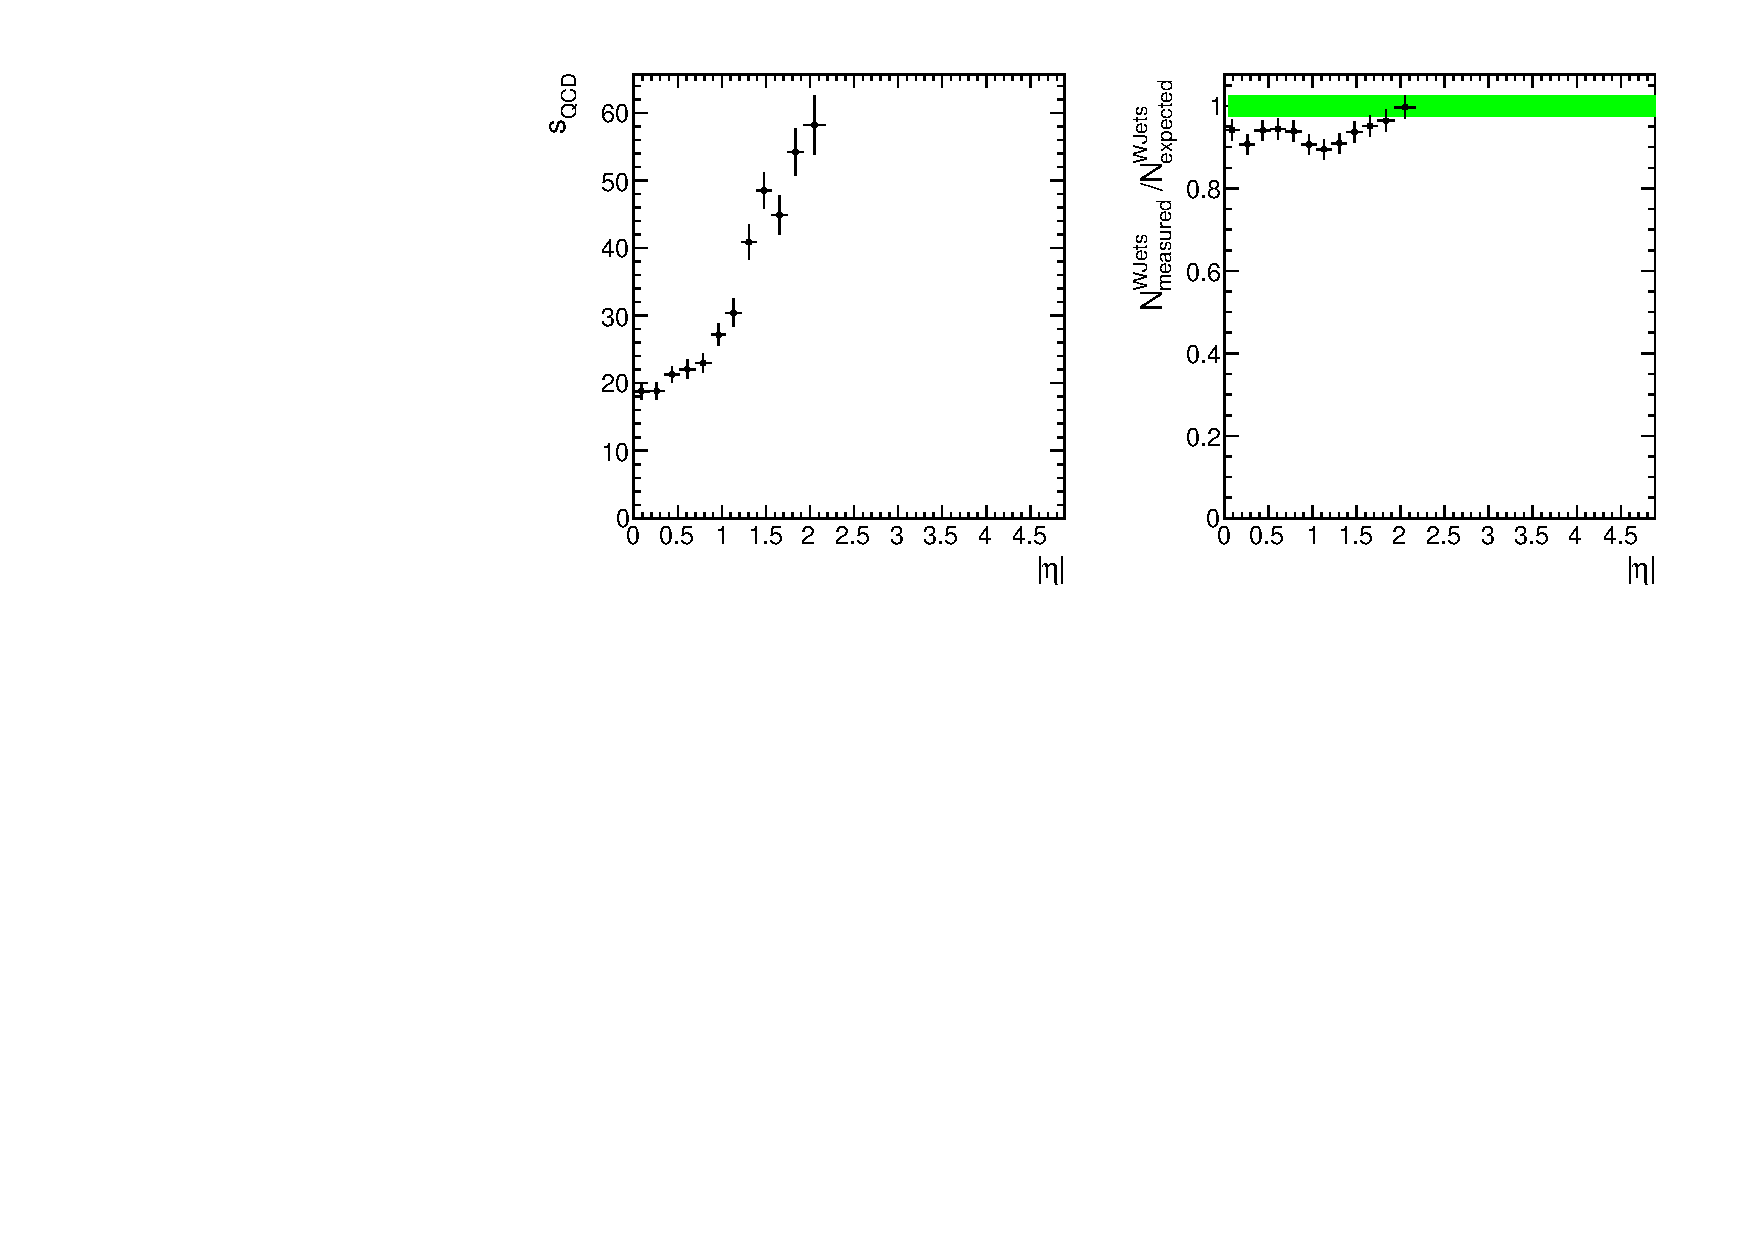
\includegraphics[width=\textwidth]{\figpath/Chapter5/QCD_EtaWeights/SfVsEta_control6_muon.pdf}
    \caption{$S_{\mathrm{QCD}}$ (left) and $S_{\Wjets}$ (right) scale factors as a function of lepton $|\eta|$ derived in the muon channel for the one jet bin. The green band indicates the uncertainty on the \Wjets expectation due to the theoretical uncertainty in the SM cross section.}
    \label{fig:SfVsEta_control6_muon}
\end{figure}

As an additional cross check, the same procedure was done to the $\geqslant$2 jets bin to see if the distribution of weights was similar to that of the control region.
From figs.~\ref{fig:AllMetFits_signal_electron} and~\ref{fig:SfVsEta_signal_electron} we see that the procedure, done on the signal region, does indeed return similar scale factors to those found in the one jet control region.
This gives us high confidence that the scale factors from the one jet bin will correct the shape of the QCD distributions in the signal region.

\begin{figure}[!hbt]
    \centering
    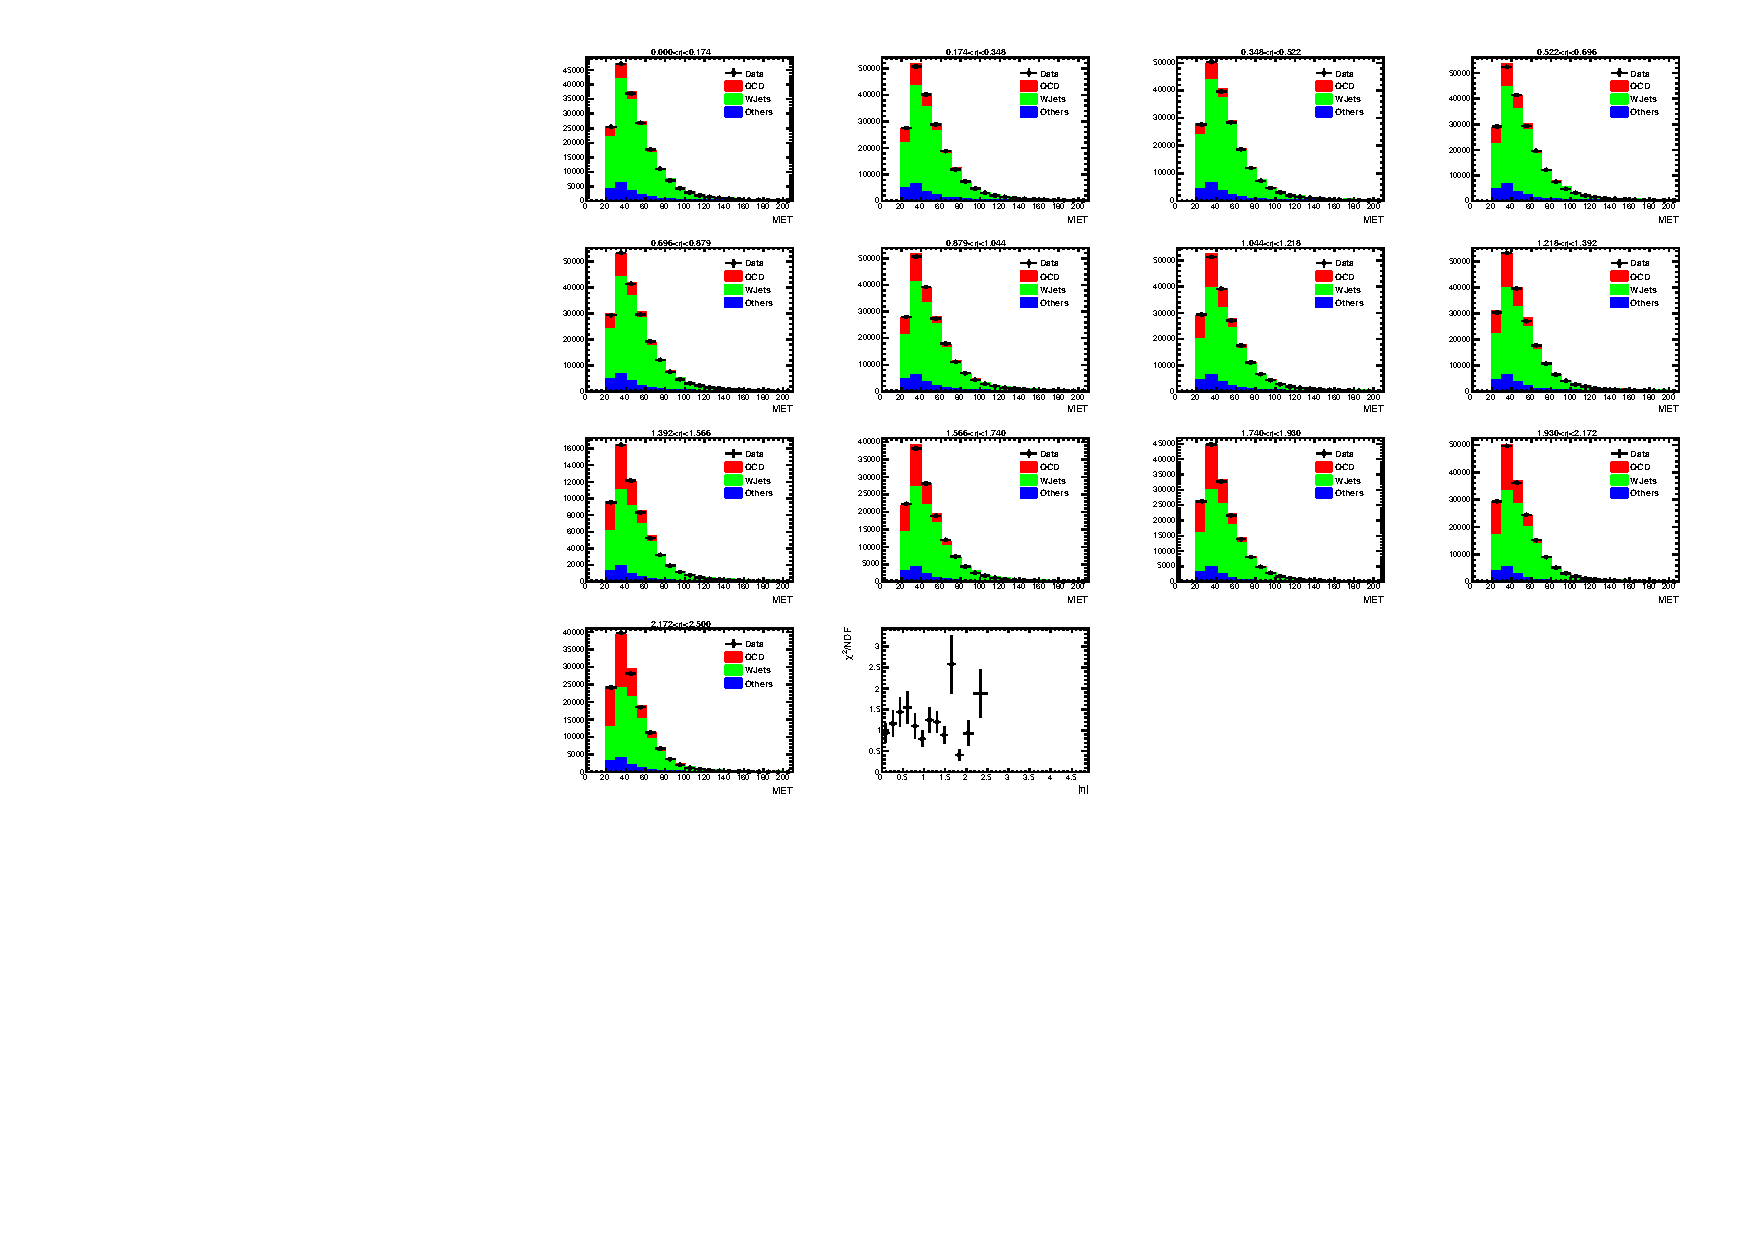
\includegraphics[width=\textwidth]{\figpath/Chapter5/QCD_EtaWeights/AllMetFits_signal_electron.pdf}
    \caption{The \ETslash distributions in the $\geqslant$2 jet bin used to derive the QCD weights in the 13 different bins of lepton $|\eta|$ after the fitting the QCD (red) and \Wjets (green) contributions to the data (black markers). The contribution from the other SM processes (blue) is held fixed to their SM expectation. The last pad in the plot show the $\chi^{2}/NDF$ of the fits.}
    \label{fig:AllMetFits_signal_electron}
\end{figure}

\begin{figure}[!hbt]
    \centering
    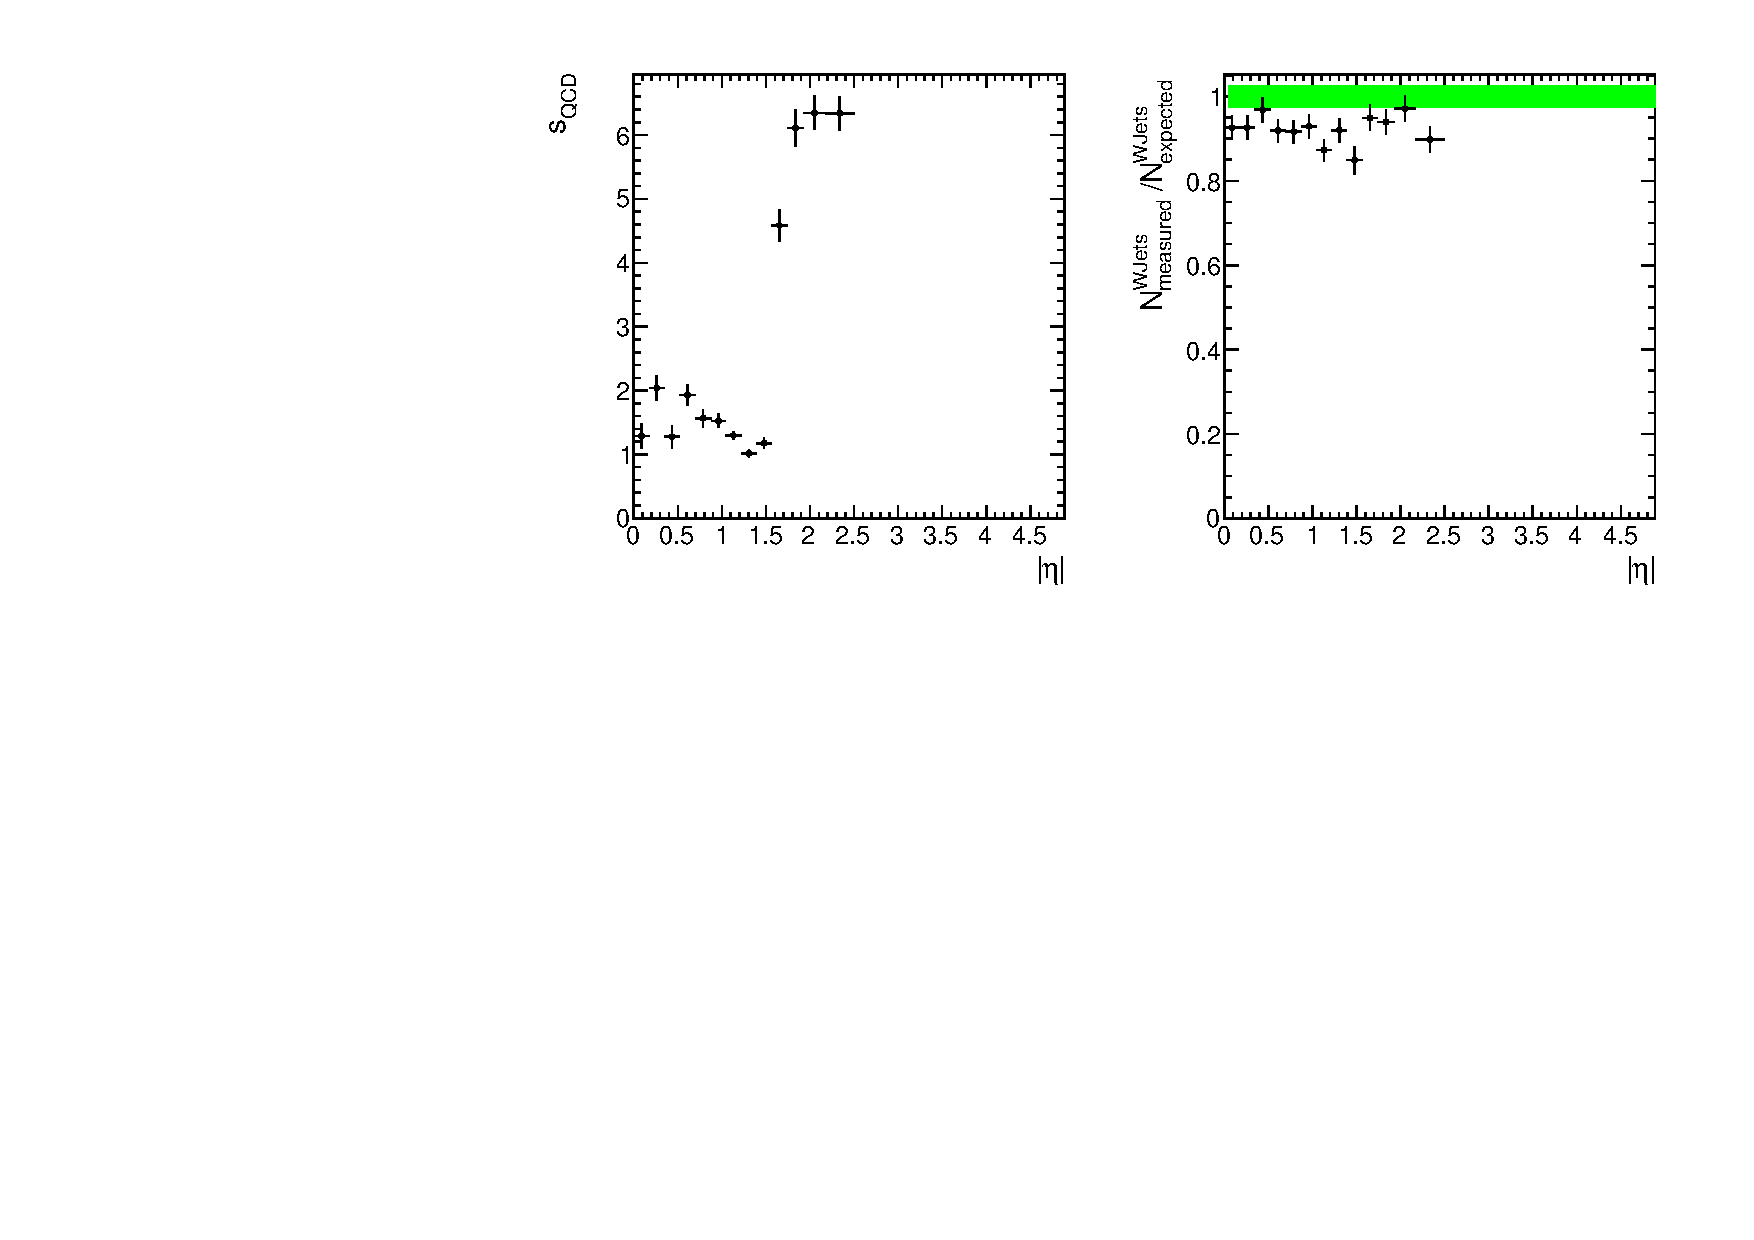
\includegraphics[width=\textwidth]{\figpath/Chapter5/QCD_EtaWeights/SfVsEta_signal_electron.pdf}
    \caption{$S_{\mathrm{QCD}}$ (left) and $S_{\Wjets}$ (right) scale factors as a function of lepton $|\eta|$ derived in the electron channel for the $\geqslant$2 jet bin. The green band indicates the uncertainty on the \Wjets expectation due to the theoretical uncertainty in the SM cross section.}
    \label{fig:SfVsEta_signal_electron}
\end{figure}

The right plot of fig.~\ref{fig:SfVsEta_signal_electron} shows that the \Wjets normalization also needs to be measured as a fit to the ratio of measured events and expected events yields a value of $0.953\pm0.008$, which is not consistent with the 2.56\% error on the theoretical cross section.
To find the correct \Wjets and QCD normalizations a two component fit to the \ETslash distribution of the data is used, allowing only the \Wjets and QCD fractions to float.
The expected yields of the other SM backgrounds are held constant during the fit.
A Gaussian constraint is imposed on the \Wjets scale factor because its theoretical cross section uncertainty is known.
The derived scale factors are shown in table~\ref{tab:WJet_QCD_ScaleFactors}.

\begin{table}[hbtp]\footnotesize
\centering
\begin{tabular}{l l l}
\hline
Lepton Category & \Wjets SF & QCD SF \\
\hline
Electron & $1.04515\pm0.00509474$ & $0.248858\pm0.0131115$ \\
Muon     & $0.969517\pm0.00442517$ & $0.145418\pm0.00669525$ \\
\hline
\end{tabular}
\caption{\Wjets and QCD scale factors as derived from a two component fit to the \ETslash distribution.}
\label{tab:WJet_QCD_ScaleFactors}
\end{table}

\section{Data-to-MC Comparisons \& Yields}

After applying all of the object and event selections, object corrections, and event weights we can now look at the expected yields for the simulated signals and backgrounds.
Table~\ref{tab:yields_KinMEBDT} shows the event yields for our signal selection separated by jet bin, but combining the electron and muon categories.
Table~\ref{tab:percent_yields_KinMEBDT}, on the other hand, shows the percentage yields where the numbers from table~\ref{tab:yields_KinMEBDT} have been normalized to the sum of the events in background and signal sections.
In both tables, Higgs events where the Higgs boson does not decay to two \W bosons are referred to as 'volunteer signal'.
This is in contrast to true \HWW events, which we sometimes refer to as 'true signal'.
Both of these categories are normalized to the \HWW yields in order to be able to compare the volunteer signal contamination to the true signal.

\begin{sidewaystable}[htbp]
\centering
\begin{tabular}{lccc} \hline
\textbf{Process} & \textbf{2 Jets} & \textbf{3 Jets} & \textbf{$\geqslant$4 Jets}\\ \hline
Diboson & $46495.97\pm78.55$ & $15049.18\pm44.70$ & $4150.48\pm23.47$ \\
\Wjets & $3446003.06\pm6434.30$ & $756463.35\pm3008.63$ & $189815.29\pm1515.40$ \\
\Zjets & $270460.62\pm822.24$ & $69061.73\pm415.90$ & $19829.24\pm222.71$ \\
\ttbar & $22452.06\pm142.85$ & $27902.44\pm160.86$ & $31218.33\pm170.54$ \\
Single \cPqt & $16587.13\pm84.31$ & $7193.89\pm59.29$ & $3068.60\pm40.25$ \\
Multijet & $275465.33\pm952.52$ & $74168.89\pm504.39$ & $22109.53\pm282.94$ \\\hline
\rowcolor{mygray}
Total Background & $4077464.17\pm6558.75$ & $949839.48\pm3083.93$ & $270191.47\pm1567.59$ \\\hline
ggH, \HWW \MH=125\gev & $552.09\pm1.92$ & $211.15\pm1.19$ & $79.51\pm0.73$ \\
qqH, \HWW \MH=125\gev & $106.60\pm0.56$ & $52.66\pm0.39$ & $17.51\pm0.23$ \\
WH\_ZH\_TTH, \HWW \MH=125\gev & $136.20\pm2.22$ & $84.35\pm1.75$ & $42.32\pm1.22$ \\\hline
\rowcolor{mygray}
Total \HWW & $794.89\pm2.99$ & $348.16\pm2.15$ & $139.34\pm1.44$ \\\hline
WH\_ZH\_TTH, \HZZ \MH=125\gev & $10.30\pm0.17$ & $5.30\pm0.12$ & $2.35\pm0.08$ \\
WH, \Hbb \MH=125\gev & $45.34\pm0.40$ & $14.22\pm0.23$ & $3.86\pm0.12$ \\
\ttH, \Hbb \MH=125\gev & $0.59\pm0.03$ & $1.33\pm0.05$ & $3.77\pm0.09$ \\\hline
\rowcolor{mygray}
Total Volunteer Signal & $56.23\pm0.44$ & $20.85\pm0.26$ & $9.98\pm0.17$ \\\hline
Signal \textsubscript{\HWW}/Bkg & 0.000195 & 0.000367 & 0.000516 \\
Signal \textsubscript{\HWW}/$\sqrt{\text{Bkg}}$ & 0.394 & 0.357 & 0.268 \\\hline
\rowcolor{mygray}
Data & $4057594$ & $953513$ & $272713$ \\\hline
\end{tabular}
\caption{Expected yields for both the electron and muon categories when normalized to the SM cross sections and collected luminosity. The table is broken up into three sections; the top section contains all of the background processes, the middle section shows the \HWW contributions, and the bottom section shows the other Higgs processes that could mimic our final state, but do not originate from a \HWW process. This table contains the yields for the zero b-tag category. Only statistical uncertainties are shown.}
\label{tab:yields_KinMEBDT}
\end{sidewaystable}

\begin{table}[htbp]
\centering
\begin{tabular}{lccc} \hline
\textbf{Process} & \textbf{2 Jets} & \textbf{3 Jets} & \textbf{$\geqslant$4 Jets}\\ \hline
Diboson & 0.011 & 0.016 & 0.015 \\
\rowcolor{green}
\Wjets & 0.845 & 0.796 & 0.703 \\
\Zjets & 0.066 & 0.073 & 0.073 \\
\ttbar & 0.006 & 0.029 & 0.116 \\
Single \cPqt & 0.004 & 0.008 & 0.011 \\
Multijet & 0.068 & 0.078 & 0.082 \\\hline
\rowcolor{mygray}
Total Background & 1.000 & 1.000 & 1.000 \\\hline
ggH, \HWW \MH=125\gev & 0.695 & 0.606 & 0.571 \\
qqH, \HWW \MH=125\gev & 0.134 & 0.151 & 0.126 \\
WH\_ZH\_TTH, \HWW \MH=125\gev & 0.171 & 0.242 & 0.304 \\\hline
\rowcolor{mygray}
Total \HWW & 1.000 & 1.000 & 1.000 \\\hline
WH\_ZH\_TTH, \HZZ \MH=125\gev & 0.013 & 0.015 & 0.017 \\
WH, \Hbb \MH=125\gev & 0.057 & 0.041 & 0.028 \\
\ttH, \Hbb \MH=125\gev & 0.001 & 0.004 & 0.027 \\\hline
\rowcolor{mygray}
Total Volunteer/Total \HWW & 0.071 & 0.060 & 0.072 \\\hline
\end{tabular}
\caption{Expected percent yields for both the electron and muon categories separated by jet bin. The background samples are normalized by the total background, while the \HWW and volunteer signal samples are normalized by the \HWW total. The Dominant background in all jet bins, \Wjets, is highlighted in green. This table contains the percent yields for the zero b-tag category.}
\label{tab:percent_yields_KinMEBDT}
\end{table}

It is clear from these tables that the dominant background for all jet bins is \Wjets.
Its expected yield is by far much larger than all of the other backgrounds.
From table~\ref{tab:percent_yields_KinMEBDT} one can also see that the sum of the volunteer signal is at most 7\% of the \HWW signal, which means the b-tag cut is keeping the non-\HWW contamination to a minimum.
If the b-tag cut was not used the \ttbar background would become much more significant, even becoming the dominant background in the $\geqslant$4 jet bin.
Additionally, the volunteer signal would become as high as 87\% of the \HWW signal, which means that there would be a lot of overlap between this analysis and other CMS analyses.

\section{Multivariate Analysis}

One of the problems of past analyses, such as cut-and-count experiments, is that they ignore the additional information that comes from using the many correlated bins of a shape analysis.
By doing a cut-and-count experiment across many bins an analysis is able to gain in discrimination power.
That being said, it would be wasteful and suboptimal to use a single discriminating kinematic distribution, which means the discrimination power of the unused variables is missed.
This analysis uses the output of a boosted decision tree (BDT) classifier as the template used for limit setting, choosing to combine the discrimination power of several kinematic variables.
This type of multivariate analysis (MVA) is useful in quantifying the separation of the signal samples (\HWW) from the background samples.

\subsection{Boosted Decision Tree}

Multivariate techniques are used to model the dependence of one or more target variables on a set of input variables.
Boosted decision trees are a more robust alternative to artificial neural networks and were first introduced to the high energy physics (HEP) community by the MiniBooNE collaboration~\cite{Roe:2004na}.
This machine learning (ML) technique has since been used countless times throughout the HEP community.
This analysis makes use of the BDT algorithm implemented in the ROOT TMVA package~\cite{1742-6596-219-3-032057}.
The key ingredient here is the boosting technique, which helps to mitigate the problem of ``overtraining,'' which is common to ML algorithms, and increases the overall performance of the algorithm~\cite{Hocker:2007ht}.
The issue with overtraining is that the output of the ML algorithm becomes overly dependent on the multivariate inputs.
In other words this means that a small change in the input variable $x{\rightarrow}x+\delta{x}$ can cause a large change in the output of the algorithm $f\left(x+\delta{x}\right)-f\left(x\right)\gg\epsilon$.
The ML algorithm may be picking up on minute changes in the simulation or statistical fluctuations, both of which are not true features of the target classification.
While these jumps may seem to indicate a higher amount of discrimination power in the training sample, they are not indicative of the underlying physics being modeled and must be suppressed.
The BDT algorithm train many weak decision trees, which are then combined using the namesake ``boosting algorithm.''
This algorithm ``boosts'' the events that are misclassified in the previous tree so that each successive generation of tree contains fewer misclassified events.
Some of the benefits of boosting are that weak or less discriminating input variables will have a reduced impact and that many input variables can be included to improve the overall classification performance.
This section will describe the general process of training of a BDT classifier while the subsequent sections will explain how the BDTs were trained for this analysis.

A decision tree is a binary tree structure made up of nodes which are meant to provide higher purity samples of signal and background at each subsequent layer of the tree.
A set of input variables is chosen by the analyzer before the start of the training sequence.
The higher purity is achieved by placing a cut on the single input variable which will achieve the best separation (highest purity) at any given node.
This can be thought of as each node creating a boundary $t\left(x\right)$ in multi-dimensional space and estimating the likelihood ratio $\frac{\mathcal{L}\left(t|S\right)}{\mathcal{L}\left(t|B\right)}$ in a small portion of that space.
The input variables should be chosen for their discrimination power, which can be quantified at each stage of the tree as $S/\left(S+B\right)$.
The signal purity $P$, on the other hand, is defined at every node as the number of signal events divided by the total number of events in the sample, both signal and background.
For purity $P$, a cut value can be chosen to minimize the Gini Index $Gini=G_{\text{left}}+G_{\text{right}}$, where $G=P\left(1-P\right)$ and $G_{\text{side}}$ is calculated one both sides of the cut.
This cut will then define the population of signal and background for two nodes in the next layer.
A perfect cut which completely separates signal from background will achieve $Gini=G_{\text{left}}=G_{\text{right}}=0$ while any impurity will mean $Gini\neq0$.
The Gini Index will reach a maximum when the samples are fully mixed.
For training purposed, the starting node will have the same mixture of signal and background as the training sample, while each successive cut level will reduce the impurity as shown in figs.~\ref{fig:BDT_Classifier_Example} and~\ref{fig:BDT_tree_HWWlvjj}.
It can be seen from both figures that a single variable may be used to define a cut at more than one node in the tree, as in the jet2dRLep variable in fig.~\ref{fig:BDT_tree_HWWlvjj}.
It is also possible that a variable will not be used at all.
The granularity of the cuts tested by the algorithm is a user specified parameter, which must be wisely chosen to allow for flexibility in the cut space, but not so granular as to adversely increase the computing time.
The stopping point of the algorithm can be based on the minimum number of training events remaining in each node, the maximum number of layers from the root node, a requirement on the purity, or a combination of two or more of those criteria.
At this point the multi-dimensional space is split into many regions, which are classified as either signal or background depending upon the purity level of the final node.
A purity $>0.5$ is classified as signal and a purity $<0.5$ is classified as background~\cite{1742-6596-219-3-032057}.

\begin{figure}[!hbt]
    \centering
    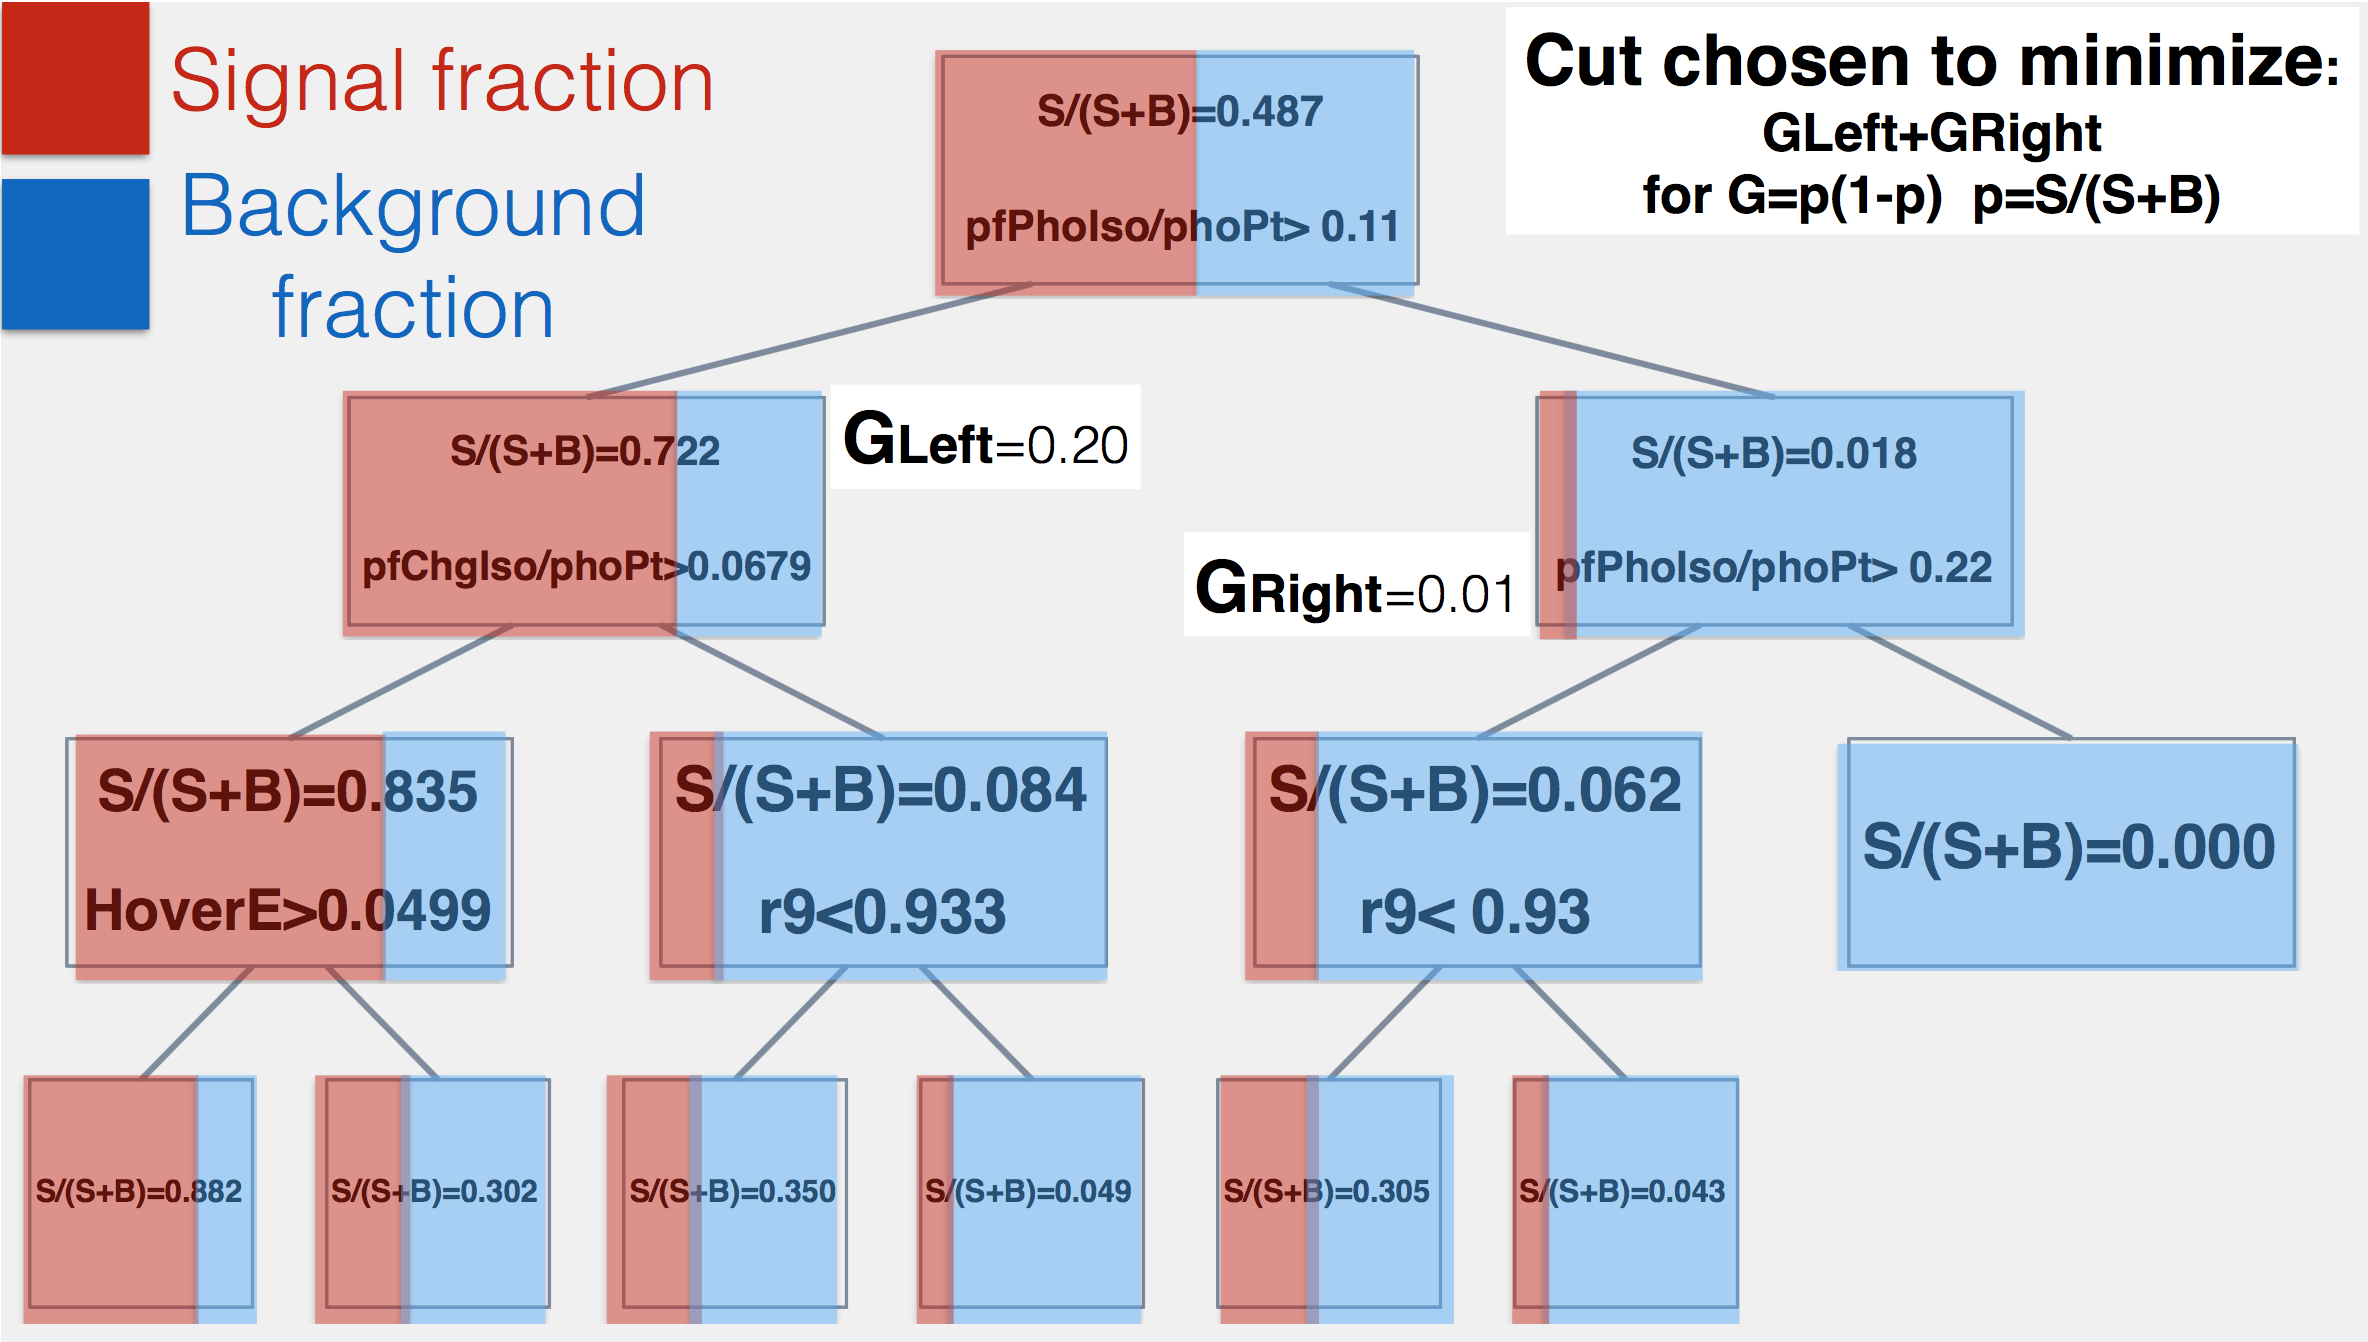
\includegraphics[width=0.95\textwidth]{\figpath/Chapter5/BDT_Classifier_Example.png}
    \caption{Example BDT classifier tree showing the cut optimization procedure to separate signal and background events. The colors within each node represent the purity $p$. The root note contains equal amounts of signal and background, but after the first layer the right-most node contains almost pure background while the left-most node contains $~$70\% signal. The base of the tree provides a node with more than 80\% signal purity.}
    \label{fig:BDT_Classifier_Example}
\end{figure}

\begin{figure}[!hbt]
    \centering
    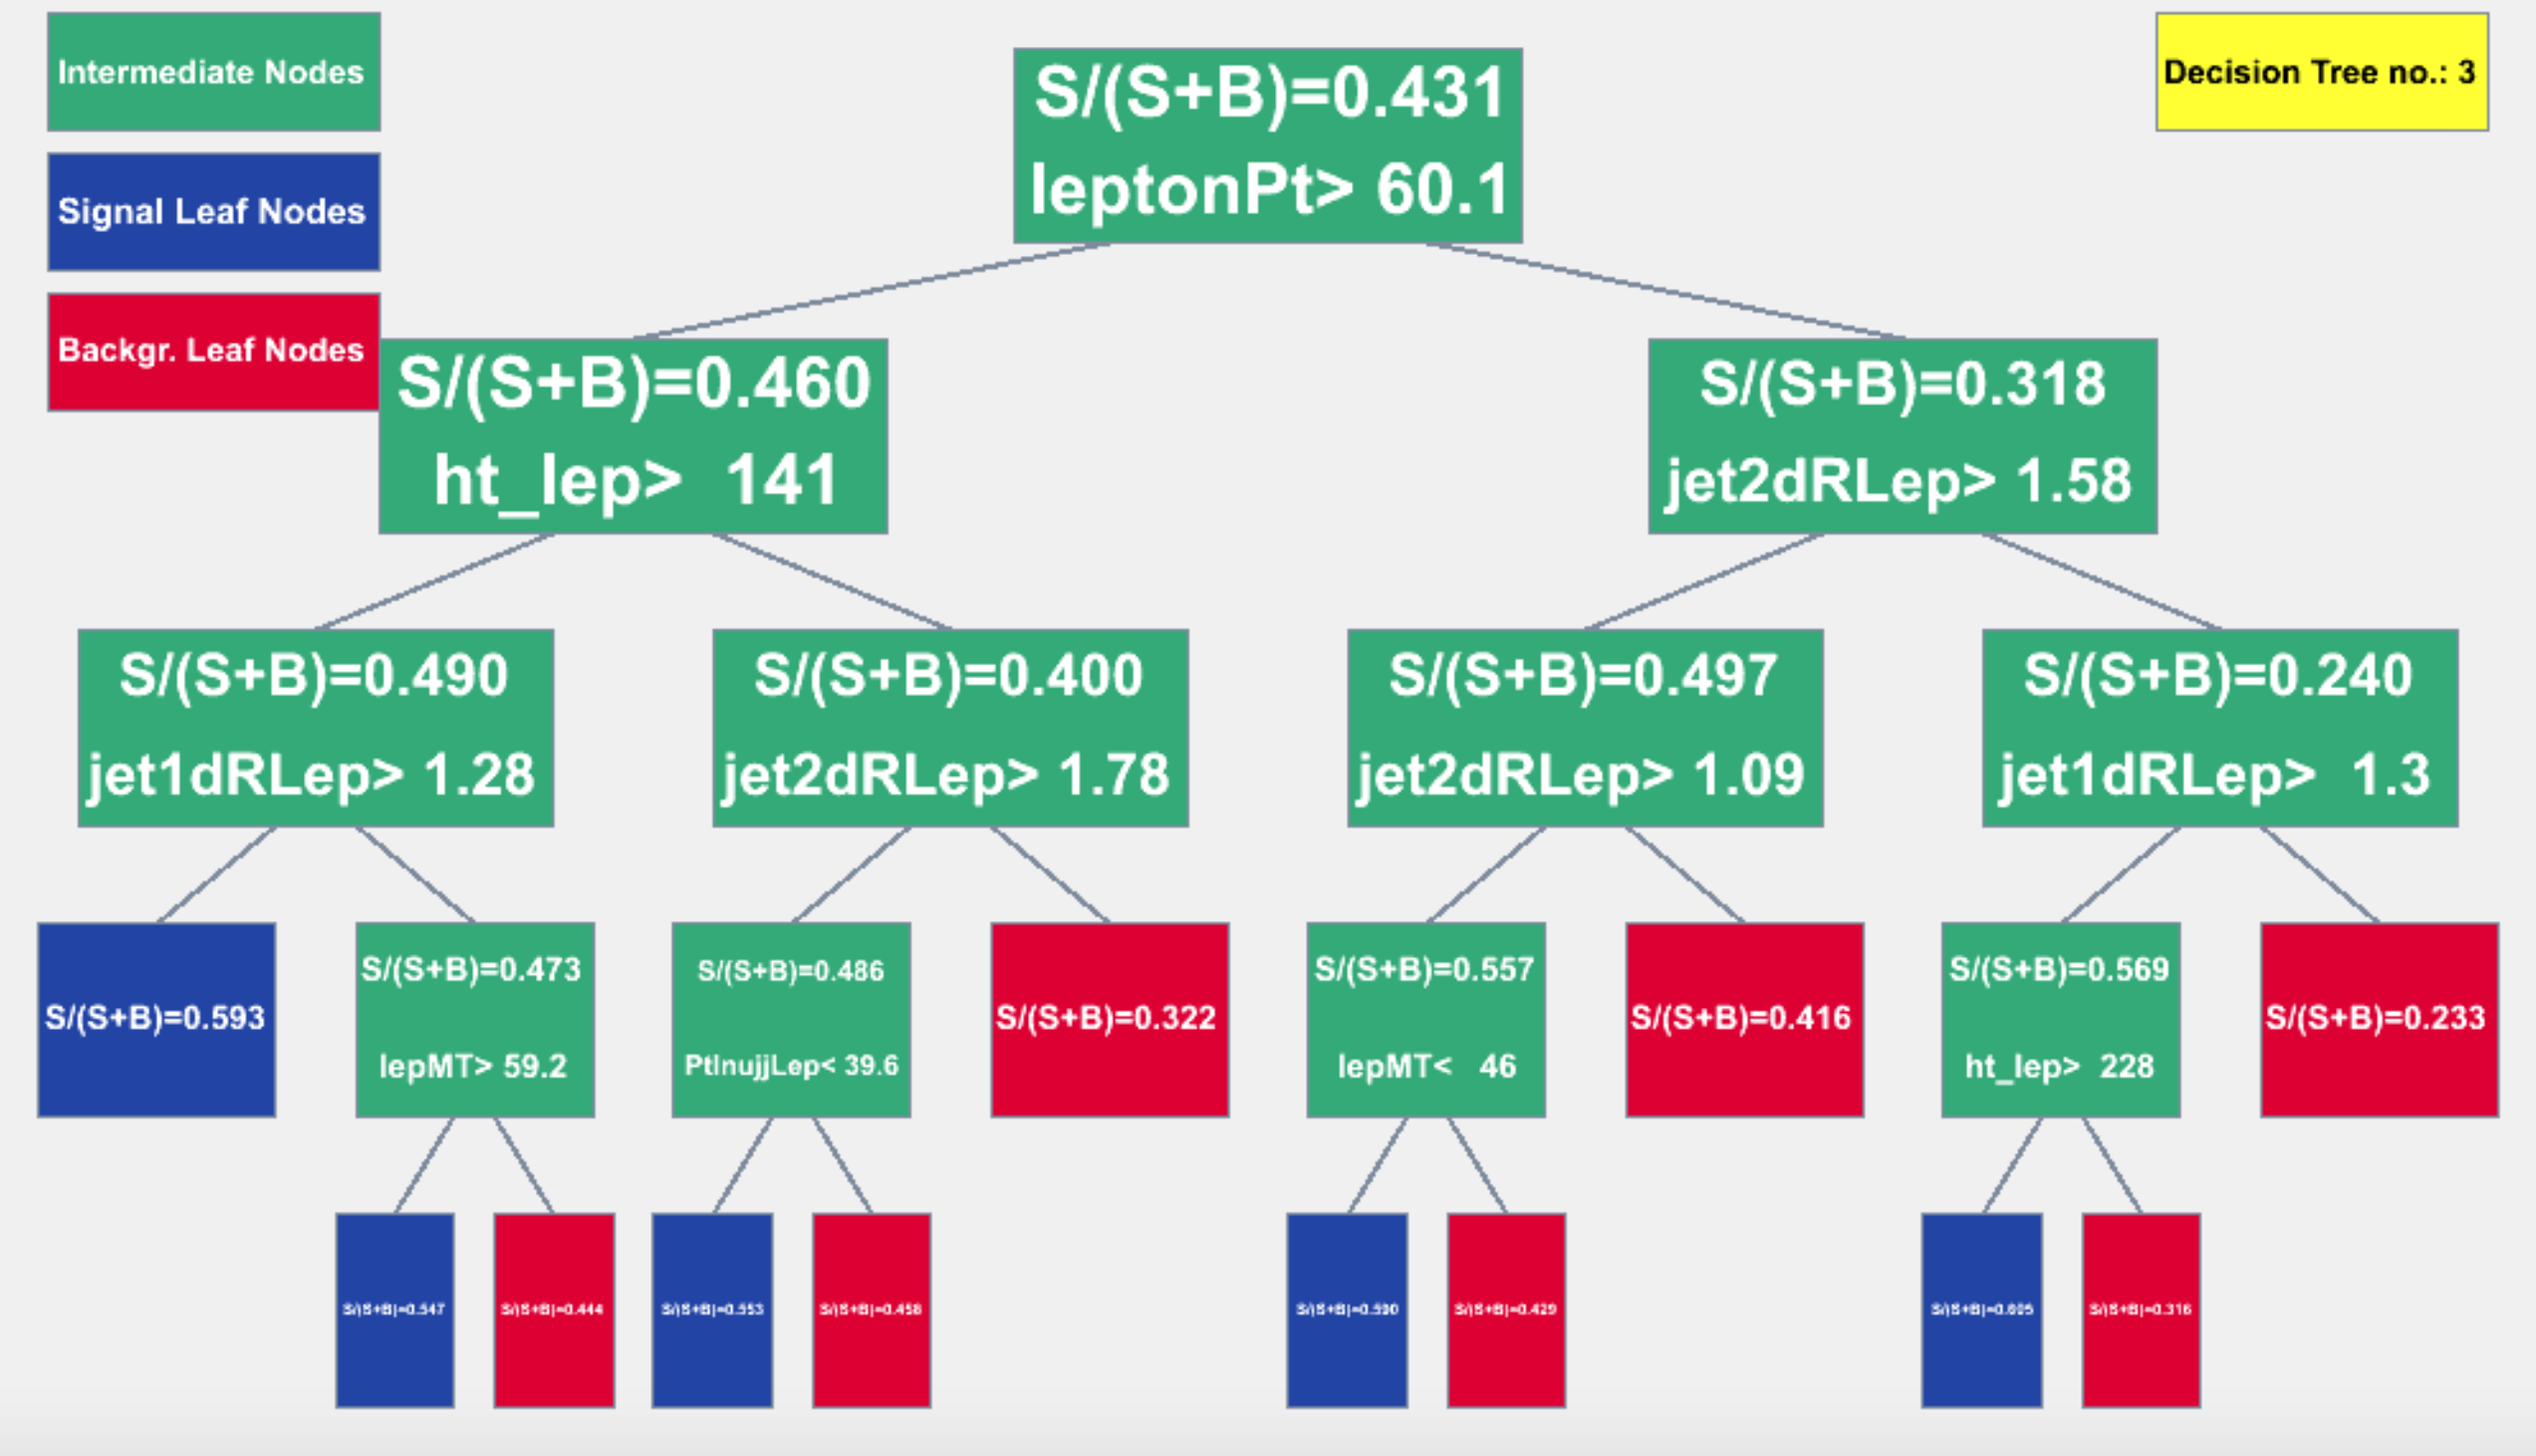
\includegraphics[width=0.95\textwidth]{\figpath/Chapter5/BDT_tree_HWWlvjj.png}
    \caption{An example decision tree used by this analysis. This tree will be combined with a forest of other trees using the boosting algorithm. The bottom nodes are defined as being more signal or background like based on the majority population left in the node.}
    \label{fig:BDT_tree_HWWlvjj}
\end{figure}

\begin{comment}
Boased on Rishi's thesis, but may only be applicable to gradient boosting

Training many independent decision trees without boosting will not prevent overtraining as each tree would have a different misclassification rate.
The boosting algorithm solves this by combining many decision trees (a ``forest'' of trees) to minimize the ensemble misclassification rate.
The weighted sum of the tree outputs is given by:
\begin{equation}\label{eq:decision_tree_weighted_sum}
  F\left(x\right)=\sum_{m=0}^{M}\beta_{m}f\left(x,a_{m}\right),
\end{equation}
where the $m$ trees are represented by base functions $f\left(x,a_{m}\right)$ and the set of values $\left(a_{m},\beta_{m}\right)$ are chosen to minimize a specially chosen loss function.
Note that $\beta_{m}$ improves the performance of the algorithm by reducing the learning rate.
The loss function choice determines the specific boosting procedure.
\end{comment}

Training many independent decision trees without boosting will not prevent overtraining as each tree would have a different misclassification rate.
The boosting algorithm solves this by combining many decision trees (a ``forest'' of trees) to minimize the ensemble misclassification rate.
This analysis makes use of the adaptive boost (AdaBoost) procedure, which weights higher in subsequent trees events which are mis-classified in the current tree~\cite{FREUND1997119}.
The event weights are initialized to 1, but change after the first tree.
Nevertheless, the weights in each tree are always normalized such that the sum of the weights remains constant.
The events in each new tree are weighted by multiplying the previous event weights by a boost weight $\alpha$ common to the tree.
$\alpha$ is defined as:
\begin{equation}
  \alpha=\frac{1-err}{err},
\end{equation}
where $err$ is the mis-classification rate of the previous tree.
%For the AdaBoost algorithm the combined weight, a modification to equation~\ref{eq:decision_tree_weighted_sum}, is given by:
The weighted sum of the tree outputs is given by:
\begin{equation}
  y_{\text{Boost}}\left(\textbf{x}\right)=\frac{1}{M}\sum_{m=0}^{M}\ln\left(\alpha_{m}\right)h_{m}\left(\textbf{x}\right),
\end{equation}
where there are $m$ trees, $\textbf{x}$ are the input variables, and $h\left(\textbf{x}\right)\in\{-1,1\}$ is the single event classifier indicating if the event is signal, $h\left(\textbf{x}\right)=1$, or background, $h\left(\textbf{x}\right)=-1$.
The resulting discriminant on the event at the end of the training, $y_{\text{Boost}}\left(\textbf{x}\right)$, is a number in the range $[1,-1]$, where 1 is most signal-like and -1 is most background-like.

The AdaBoost procedure is ideal for use with shallow trees with two or three levels each, leaving a relatively large population of events in each of the final nodes.
These are also known as weak classifiers and provide little discrimination power on their own.
The benefit to using these is that they are much less prone to overtraining, but they can be grouped together, through the boosting procedure, to provide good discrimination power.
Had the trees been allowed to reach a state where a single event was left in a node, this would imply that there was a cut sequence that would lead to perfect signal versus background classification, a practical impossibility.
It is therefore important that the analyzer keep this in mind when specifying the stopping hyper-parameters.
One of the other hyper-parameters specific to the AdaBoost procedure is the boost weight exponent, where $\alpha{\rightarrow}\alpha^{\beta}$.
By changing $\beta$ one can slow down the learning rate, allowing for a larger number of boost iterations.
The list of tunable hyper-parameters is as follows:
\begin{itemize}
  \item NTrees: The number of trees in the forest.
  \item nEventsMin: The minimum number of events allowed in a node after the splitting.
  \item MaxDepth: The maximum number of levels in the tree aside from the root node.
  \item BoostType: The boosting method to use. This analysis used the adaptive boost (AdaBoost) method, but other options are available.
  \item AdaBoostBeta: The exponent of the AdaBoost weight. This analysis used $\beta=0.5$.
  \item SeparationType: While this analysis used the Gini Index there are other choices for measuring the separation of signal and background.
  \item nCuts: The number of steps available for a single variable when determining the cut value. Increasing this number leads to finer granularity, the benefit of which was not seen by this analysis. We chose to use a step size of 20.
  \item PruneMethod: It is possible to prune away some branches to increase performance. This was unnecessary for this analysis as it used a boost procedure which limited the size of the tree.
  \item NodePurityLimit: This parameter determines at which purity ($P>\text{NodePurityLimit}$) the final node is considered a signal node. This analysis used a value of 0.5.
\end{itemize}

As an additional way to check for overtraining, one can reserve a set of events to use as a testing sample to check the efficacy of the classifier response.
The amount of signal and background to split off is tunable, but this analysis used half of the events for training and the other half for testing.
When comparing the training and testing distributions the Kolomogrov-Smirnoff test\footnote{The value returned by this test is the probability that the two distributions originated from the same probability distribution.} is used to determine their compatibility.
For this analysis a separate BDT is trained for each jet category and is individually optimized based on the chosen input variables and the hyper-parameters of the training algorithm.
Section~\ref{sec:kin_var_sel} will discuss the selection of the potential kinematic variables while sections~\ref{sec:BDT_input_optimization} and ~\ref{sec:BDT_parameter_optimization} will discuss the optimization of the inputs and parameters, respectively, for the individual trainings.

\subsection{Kinematic Variable Selection}
\label{sec:kin_var_sel}

While it may be tempting to use the 4-vectors of the final state objects as inputs to the BDT, shallow networks, like the ones used here, are not very good at learning the intricacies necessary to discriminate physics processes based on simple inputs.
Conversely, networks can be subject to sever overtraining if too many high level variables are used as input.
Instead, the user must choose a select set of input distributions to use, preferably ones that already has some separation between the signal(s) and  background(s).
It is also a good idea to provide the BDT only the dominant signal and background to train on, so as to develop a classifier with the maximal amount of separation power.
Given table~\ref{tab:yields_KinMEBDT} we used the normalized \Wjets background and \HWW signal MC as input samples.
A list of variables with possible separation powers was then created.
Each variable's separation power was quantified using the two figures of merit (FOM) listed in equation~\ref{eq:BDT_FOM1} and~\ref{eq:BDT_FOM2}, where $i$ denotes the bin number in the distribution.
\begin{align}
  FOM1 = {}& \sum_{i=1}^{nBins}\left(\text{signal}-\text{background}\right)^{2}\label{eq:BDT_FOM1}\\
  FOM2 = {}& \sum_{i=1}^{nBins}\frac{\left(\text{signal}-\text{background}\right)^{2}}{\left(\text{signal}+\text{background}\right)^{2}}\label{eq:BDT_FOM2}
\end{align}
Fig.~\ref{fig:BDT_FOM} shows several of these distributions with their associated figures of merit.

\begin{figure}[!hbt]
    \centering
    \begin{subfigure}[t]{0.48\textwidth}
        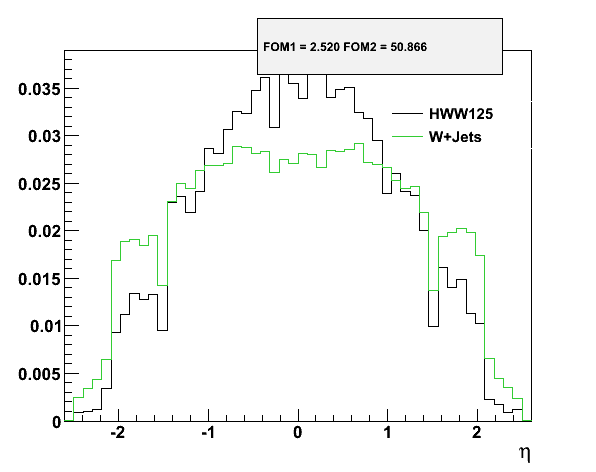
\includegraphics[width=\textwidth]{\figpath/Chapter5/BDT_InputVarOpt/lepEta.png}
        \caption{}
        \label{fig:BDT_FOM_lepEta}
    \end{subfigure}
    \begin{subfigure}[t]{0.48\textwidth}
        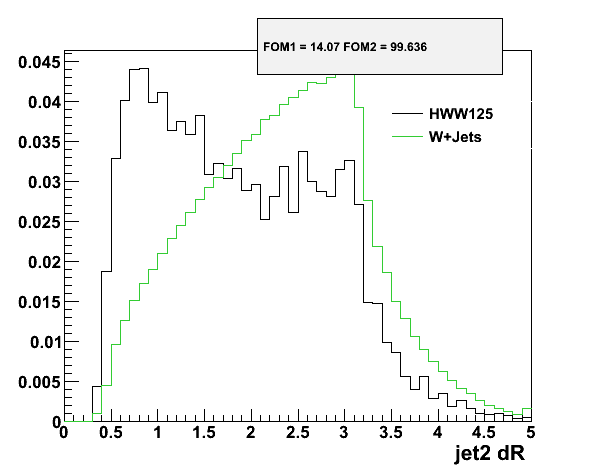
\includegraphics[width=\textwidth]{\figpath/Chapter5/BDT_InputVarOpt/jet2dRLep.png}
        \caption{}
        \label{fig:BDT_FOM_DeltaRLepJet}
    \end{subfigure}

    \begin{subfigure}[t]{0.48\textwidth}
        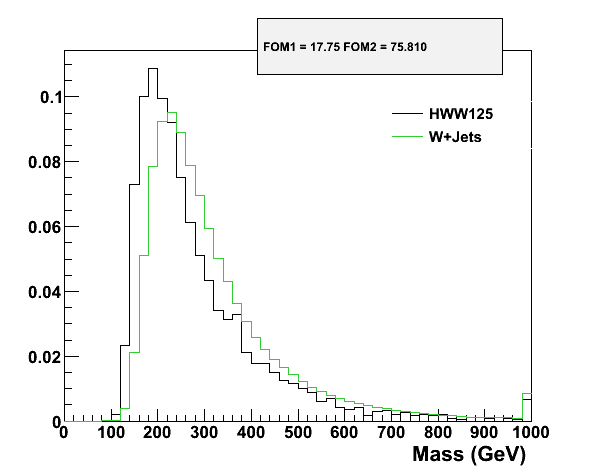
\includegraphics[width=\textwidth]{\figpath/Chapter5/BDT_InputVarOpt/MWWTop2jets.png}
        \caption{}
        \label{fig:BDT_FOM_Mlvjj}
    \end{subfigure}
    \begin{subfigure}[t]{0.48\textwidth}
        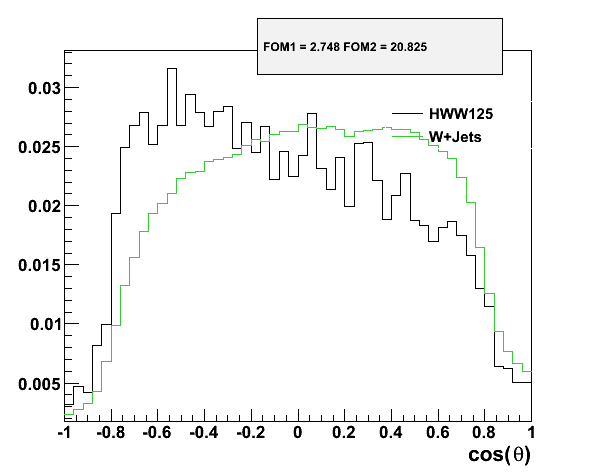
\includegraphics[width=\textwidth]{\figpath/Chapter5/BDT_InputVarOpt/CosTheta_l.png}
        \caption{}
        \label{fig:BDT_FOM_CosThetaL}
    \end{subfigure}
    \caption{Example distributions used to examine possible input variables to the BDT trainings. The \ggH (black) and \Wjets (green) samples are both unit normalized. The two FOMs calculated are shown, but since these are normalized distributions the resulting numbers would be quite small. Thus the FOM have been multiplied by $10^{5}$ for ease of reading. The four distributions are (a) lepton $\eta$, (b) $\DR\left(\Pl,\text{jet2}\right)$, (c) \Mlvjj, and (d) \costhetal.}
    \label{fig:BDT_FOM}
\end{figure}


\begin{figure}[!hbt]
    \centering
    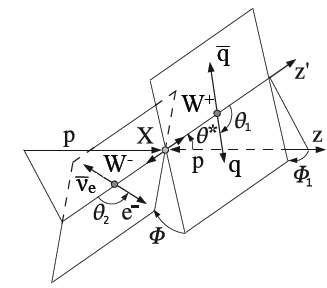
\includegraphics[width=0.95\textwidth]{\figpath/Chapter5/WDecayAngles.png}
    \caption{Planes and angular variables in the \HWWlvqq decay process~\cite{PhysRevD.81.075022}.}
    \label{fig:XWWDecayAngles}
\end{figure}






























































\subsection{BDT Input Optimization}
\label{sec:BDT_input_optimization}
\subsection{BDT Parameter Optimization}
\label{sec:BDT_parameter_optimization}
\subsection{Signal Extraction Methods}

\section{Matrix Element Analysis}
Matrix Element Method (MEM)

BDT analyses often rely on shallow networks, which are bad at finding non-linear functions

The Matrix Element Method (MEM) takes into account all final state particle kinematics and correlations
MEMs give an estimate, probability density Pi , that an event with a given final state comes from process i

\begin{comment}
Table~\ref{tab:FinalYields} clearly shows that the total signal, in every channel, is smaller than even the statistical uncertainty of the background.
A cut and count experiment will not lead to any significant results.
The previous \HWWlnujj analyses have performed a fit to sensitive distributions like the 4-body mass, the mass of the two jet plus lepton plus \ETslash system.
However, this approach only includes a small amount of information available, leaving out additional sensitive kinematic distributions.
It is also felt that a BDT analysis using only kinematic variable would be sub-optimal because shallow classifiers are not robust against non-linear correlations and are only as good as the input variables.

Instead, this analysis uses a matrix element method (MEM), which starts from the differential cross section calculation from quantum field theory to classify how likely and event is to come from a given process~\cite{Canelli2003,Dong2008}.
The probability $P\left(x;\alpha\right)=P_{evt}$ of a signal is proportional to the differential production cross section, where $\alpha$ is the parameter we wish to measure and x is a set of physical variables.
This is true if the detector resolution is sufficiently small and the beam energies are well known, as it is in the case of CMS.
In general the differential cross section can be written as~\cite{Olive:2016xmw}:
\begin{equation}\label{eq:differential_production_cross_section}
d\sigma=\frac{\left(2\pi\right)^{4}|\mathcal{M}|^{2}}{4\sqrt{\left(q_{1}\cdot{q_{2}}\right)^{2}-m_{q_{1}}^{2}m_{q_{2}}^{2}}}d\Phi_{n}\left(q_{1}+q_{2};p_{1},...,p_{n}\right)
\end{equation}
where $|\mathcal{M}|$ is the Lorentz invariant matrix element (ME); $q_{1}$, $q_{2}$ and $m_{1}$, $m_{2}$ are the 4-momenta and masses of the incident particles; $p_{i}$ are the 4-momenta of the final state particles; and $d\Phi_{n}$ is the n-body phase space.
The phase space term is written as:
\begin{equation}
d\Phi_{n}\left(q_{1}+q_{2};p_{1},...,p_{n}\right)=\delta^{4}\left(q_{1}+q_{2}-\sum_{i=1}^{n}p_{i}\right)\prod_{i=1}^{n}\frac{d^{3}p_{i}}{\left(2\pi\right)^{3}2E_{i}}
\end{equation}
After accounting for unmeasured or mis-measured particles and normalizing to the total cross section to form an event probability, equation~\ref{eq:differential_production_cross_section} becomes:
\begin{equation}
P(x;\alpha)=\frac{1}{\sigma}\int2\pi^{4}|\mathcal{M}|^{2}\frac{f\left(x_{1}\right)}{|E_{q_{1}}|}\frac{f\left(x_{2}\right)}{|E_{q_{2}}|}W\left(y,x\right)d\Phi_{4}dE_{q_{1}}dE_{q_{2}}
\end{equation}
where $f\left(x_{i}\right)$ are the PDFs, $x_{i}=E_{q_{i}}/E_{beam}$ is the fraction of the proton momentum carried by the incident parton $i$, and $W\left(y,x\right)$ is the transfer function mapping measured jet energies $x$ to the parton energies $y$ (accounts for the jet resolution of CMS).

Fifteen probabilities $P(x;\alpha)$, corresponding to the leading order diagrams of the major background and signal processes, are computed for each event. 
This computation is by far the most time consuming aspect of this analysis, consuming $\sim$12 million CPU hours.
The information contained in these 15 probabilities must be combined in order to discriminate signal from background.
\end{comment}


\subsection{Differential Cross Section}
\subsection{Parton Distribution Functions and Phase Space}
\subsection{Transfer Functions}
\subsection{Combinatorial Considerations}
\subsection{Numerical Integration}
\subsection{Matrix Element Computation}
\subsection{Standalone BDT}
\subsection{Combined BDT}

\begin{comment}
In order to combine the complimentary information from the kinematic variables and the MEs, with the purpose of discriminating a Higgs event from a background event, we used several Boosted Decision Trees (BDTs).
An initial BDT was computed which combined the information from 15 of the computed MEs.\footnote{A BDT was used rather than combining the ME into a likelihood as in the Matrix Element Likelihood Analysis (MELA) used by H$\rightarrow$ZZ$\rightarrow$4l or using some basic ratios of signal over background probabilities as was done by CDF.}
This gives a less discriminating shallow network the ability to create a better performing network because the inputs are already non-linear variables.
The output of this BDT, along with several carefully selected kinematic variables, is then used as the input to a new BDT in order to combine all of this complimentary information.
While it may seem that the MEs should encode all of the event information perfectly, only the leading MEs were used and the permutations of the jets and partons degrades the discrimination power of the MEs.
The combined BDT has more discrimination power than either the MEs or the kinematic variables alone. 

A distribution of the BDT discriminant is produced for every signal, background, and data sample and then passed to the RooStats-based Higgs Combine Tool~\cite{CombineToolTwiki} to compute limits on the Higgs signal strength.
Given that this analysis has a relatively high number of events in the expected yields we make use of the asymptotic method\footnote{If there had been a lower number of expected events we may have needed to use the full frequentist method rather than the asymptotic method.} for limit setting along with the CL\textsubscript{s} test statistic~\cite{Read:2002hq}.
Using an Asimov dataset an expected 95\% upper confidence level is obtained and shown in figure~\ref{fig:limits} (left).
\end{comment}

original bin width 0.02 [-1,1]
bin must have background events
stat error must be less than 10\%
bins merged left to right until all bins meet this criteria
limited or no background in a bin would lead to an inflated signal significance if data, but no background

\section{Systematic Uncertainties}
TURN THESE SUBSECTIONS INTO BOLDED PARAGRAPH HEADERS

\subsection{Jet Energy Scale}
\subsection{Lepton Selection and Trigger Efficiency}
\subsection{W+jets Shape Uncertainties}
\subsection{Pileup Weights}
In order to assess the effect of a systematic uncertainty due to choice of $\sigma_{\text{inelastic}}=69.3\unit{mb}$, a $\pm$7\% variation was used.
\subsection{CSV Weights}
\subsection{Top \texorpdfstring{$p_{T}$}{pT}}
\subsection{LHC Luminosity}
\subsection{Sample Cross Sections}
\subsection{MET Uncertainty }
\subsection{QCD \texorpdfstring{$\eta$}{eta} Weights Uncertainty}
\subsection{Summary of Systematics}

\begin{comment}
Given that this is a shape analysis, it is important to consider systematic uncertainties that may change the expected yields (rate changes), the shape of the discriminating variable, or both.
This analysis considers all three of these, but decouples the rate and shape changes during limit setting.
Table~\ref{tab:ListOfSystematics} summarizes all of the systematic uncertainties considered for this analysis.
Changes to the limits greater than 1\% come from the scheme used to reweight the $\eta$ distribution in the QCD sample, the jet energy scale, the $\cos\left(\theta_{l}\right)$ weights, and the lepton efficiency uncertainty.
There will be much more detail on each of the systematics in the thesis.

\begin{table}[htbp]
  \centering
  \noindent
  \small
    \captionsetup{width=.85\textwidth}
    \caption*{Systematic Uncertainties for H$\rightarrow$WW$\rightarrow$l$\nu$jj Analysis}
    \begin{tabular}{|l|c|c|c|} \hline
Uncertainty & Rate (Y/N) 2 & Shape (Y/N) & Comments \\ \hline
$Q^{2}$ Scaling & Y & Y & W+jets MC only \\ \hline
ME/PS Matching & Y & Y & W+jets MC only \\ \hline
Background xSec & Y & N & All background samples \\  \hline
Signal xSec & Y & N & All signal MC samples \\  \hline
Luminosity & Y & N & All samples \\  \hline
MC Pileup reweighting & Y & N & All MC samples \\  \hline
Trigger Efficiency & Y & N &  All MC samples\\  \hline
Lepton Selection Efficiency & Y & N & All MC samples\\  \hline
JES Uncertainties & Y & Y & All MC samples \\  \hline
Met Uncertainty & Y & N & All samples\\  \hline
CSV Reshaping & Y & N &  All MC samples\\  \hline
Top Pt-reweighting & Y & Y &  TTbar MC only\\  \hline
QCD $\eta$ Weight & Y & Y & QCD shape, W+jets and QCD rate \\ \hline
$\cos\left(\theta_{l}\right)$ Weight & N & Y & W+jets MC only \\ \hline
    \end{tabular}
    \caption{List of all systematic uncertainties applied in analysis, whether that uncertainty has a rate or shape component to it, and which samples is is applied to.}
    \label{tab:ListOfSystematics}
\end{table}
\end{comment}